\documentclass[whitelogo]{tudelft-report}
\usepackage{natbib}
\usepackage{changes}
\usepackage{amsthm}
\usepackage{algorithm}
\usepackage{subcaption}
\usepackage{multirow}
\usepackage{booktabs}
\usepackage[noend]{algpseudocode}


\theoremstyle{plain}
\newtheorem{thm}{Theorem} % reset theorem numbering for each chapter
\newtheorem{cor}{Corollary}
\newtheorem{lem}{Lemma}
\newtheorem{pol}{Policy}

\theoremstyle{definition}
\newtheorem{defn}{Definition} % definition numbers are dependent on theorem numbers
\newtheorem{exmp}{Example} % same for example numbers
\newtheorem{prop}{Property} % same for example numbers


\begin{document}

%% Use Roman numerals for the page numbers of the title pages and table of
%% contents.
\frontmatter

%% Uncomment following 19 lines for a cover with a picture on the lower half only
%\title[tudelft-white]{Title}
%\subtitle[tudelft-cyan]{Optional subtitle}
%\author[tudelft-white]{J.\ Random Author}
%\affiliation{Technische Universiteit Delft}
%\coverimage{cover.jpg}
%\titleoffsetx{10cm}
%\titleoffsety{10cm}
%\afiloffsetx{1cm}
%\afiloffsety{18cm}
%\covertext[tudelft-white]{
%    \textbf{Cover Text} \\
%    possibly \\
%    spanning 
%    multiple 
%    lines
%    \vfill
%    ISBN 000-00-0000-000-0
%}
%\makecover

%% Uncomment following 16 lines for a cover with a picture on the lower half only
% \title[tudelft-white]{Towards global consensus on trust}
% \subtitle[tudelft-black]{Aggregation of temporal PageRank trust vectors}
% \author[tudelft-white]{J.\ Harms}
% \affiliation{Technische Universiteit Delft}
% \coverimage{cover.jpg}
% \setpagecolor{tudelft-cyan}
% \makecover[split]


%% Include an optional title page.
% \begin{titlepage}


\begin{center}

%% Insert the TU Delft logo at the bottom of the page.

%% Print the title in cyan.
{\makeatletter
\largetitlestyle\fontsize{64}{94}\selectfont\@title
%\largetitlestyle\color{tudelft-cyan}\Huge\@title
\makeatother}

%% Print the optional subtitle in black.
{\makeatletter
\ifx\@subtitle\undefined\else
    \bigskip
   {\tudsffamily\fontsize{22}{32}\selectfont\@subtitle}    
    %\titlefont\titleshape\LARGE\@subtitle
\fi
\makeatother}

\bigskip
\bigskip

by
%door

\bigskip
\bigskip

%% Print the name of the author.
{\makeatletter
%\largetitlefont\Large\bfseries\@author
\largetitlestyle\fontsize{26}{26}\selectfont\@author
\makeatother}

\bigskip
\bigskip

to obtain the degree of Master of Science
%ter verkrijging van de graad van Master of Science

at the Delft University of Technology,
%aan de Technische Universiteit Delft,

to be defended publicly on Tuesday January 1, 2013 at 10:00 AM.
%in het openbaar de verdedigen op dinsdag 1 januari om 10:00 uur.

\vfill

\begin{tabular}{lll}
    Student number: & 1234567 \\
    Project duration: & \multicolumn{2}{l}{March 1, 2012 -- January 1, 2013} \\
    Thesis committee: & Prof.\ dr.\ ir.\ J.\ Doe, & TU Delft, supervisor \\
        & Dr.\ E.\ L.\ Brown, & TU Delft \\
        & Ir.\ A.\ Aaronson, & Acme Corporation
\end{tabular}
%% Only include the following lines if confidentiality is applicable.

\bigskip
\bigskip
\emph{This thesis is confidential and cannot be made public until December 31, 2013.}
%\emph{Op dit verslag is geheimhouding van toepassing tot en met 31 december 2013.}

\bigskip
\bigskip
An electronic version of this thesis is available at \url{http://repository.tudelft.nl/}.
%\\[1cm]

%\centering{
\includegraphics{cover/logo_black}}


\end{center}

\begin{tikzpicture}[remember picture, overlay]
    \node at (current page.south)[anchor=south,inner sep=0pt]{
        
\includegraphics{cover/logo_black}
    };
\end{tikzpicture}

\end{titlepage}



% \chapter*{Preface}
\setheader{Preface}

The big hype around Bitcoin and other cryptocurrencies seems to create a distorted picture of the 
original idea of a distributed, democratic financial system. The general public does not appreciate
the simplicity and brilliance of the concept but rather the price swings and the
possibility to become rich. 

A similar distortion happened to the internet itself. Once envisioned as an 
open and free network for information exchange, the World Wide Web has been transformed into an
infrastructure for commerce, data collection and cyber attacks. Certainly, many companies have created 
solutions that simplify our lives significantly. But the free use of all kinds of services comes at 
an invisible cost. Slowly, that cost becomes more visible as targeted misinformation campaigns are
dismantling democracies and data collection policies of the big internet monopolies are uncovered.

Decentralization is a natural solution to this problem. Some fundamental services such as transferring
money, communication and the access to information should not be controlled by single entities and 
exploited for profit. In the same sense, creating trust with other internet users should be 
enabled through a decentralized system. This is the motivation to contribute to the design of a
distributed trust system.

Working on this thesis has been a journey through many fields of science, from evolution theory and 
social sciences to synchronization methods of replicated databases. 
It has in many ways opened my eyes to the problems of centralized 
organizations and the advantages that distributed systems offer. Also, it sparked my interest in 
trust, cooperation and their relation to problems of society.

I would like to thank my supervisor Dr.\ Johan Pouwelse for his enthusiasm, infinitely large pool of
ideas and suggestions as well as his invaluable feedback. I thank the Tribler team for keeping me 
awake with coffee and the review work of Quinten and Martijn. I thank my parents, my girlfriend, Lyla, 
and my closest friends for their support in moments of self-doubt. A special thanks goes to my 
housemates Marnix and Liesette who helped me through the last weeks. I would also like to thank 
Alexander for our interesting talks at lunch. Without you it wouldn't have been possible.


\begin{flushright}
{\makeatletter\itshape
    \@author \\
    Delft, August 2018
\makeatother}
\end{flushright}



% \tableofcontents

%% Use Arabic numerals for the page numbers of the chapters.
\mainmatter

\chapter{Introduction}
\label{chap:introduction}
% \subtitle{Building a distributed reputation system as the basic infrastructure for creating trust 
% between relative strangers for the future digital economy.}

% \paragraph{Abstract.} Trust enables cooperation which in the long-term increases welfare for all 
% parties, but centralization creates an unhealthy information and, thus, power asymmetry. The future 
% digital economy will be driven by global cooperation between relative strangers; that cooperation 
% will be facilitated by distributed reputation systems without central ownership or control. This 
% work extends the scalable TrustChain fabric with an explicit, unambiguous, public representation of 
% the entities' states, thereby making sharing of information incentive-compatbile and putting another
% pillar for the trustful internet in place.

% 1. Since the ground-breaking work of Darwin we know that evolution of species is guided by natural selection, so mutation and inheritance lead to the strongest variation surviving. However, the classic view of the strongest survives does not explain how cooperation can occur, which requires some sort of altruism. Game theory explains …
%  Nowak, Axelrod, 

Trust is the bedrock of society. From the evolution of species, global markets all the way to the 
modern sharing economy, trust has always had an important impact on almost every aspect of our lives.
Trust is built on a good reputation which in turn is created through positive outcomes of past 
interactions. The value of a good reputation also depends on how widely known that reputation is.
In small communities, knowledge about each other is gained through gossiping or personal experience. 
But local communities become less important as global communities and marketplaces become more common
through internet based applications. Still, or even more so, those internet communities depend on 
trust. Protecting and distributing the knowledge about interactions in the digital world is a tough
challenge we are faced with when designing a global trust system.

The current state-of-the-art trust building systems are online platforms for the sharing economy.
The reputation systems of Uber\footnote{https://uber.com} and AirBnB\footnote{https://airbnb.com} are
an essential part of their business. The good reputation allows commuters to trust their driver and
get into the car of a stranger, or allows house owners to rent their home to a couple from the other
side of the world. The reputation of drivers and renters are stored on the platforms, they are both
valuable to the people as well as the company. This leads to problems when renters do not agree with
updates to the platform: they cannot take their reputation and move to a competitor. Users are locked
into those platform, giving platforms great power and influence. 

A similar situation exists in the banking world. Banks are entrusted with their clients money, but 
their power led to corruption and the trust was abused. The situation escalated in the 2007-08 
financial crisis which led to a global recession. The crisis inspired a new solution: Bitcoin. Bitcoin
is supposed to enable secure payments without banks. As such it removes power from financial 
institutions and puts it back into the hands of the actual owners of the money. 

Not every digital money transaction should require a bank, and similarly not every trustful
interaction on the internet should require a third-party. Instead, the ability to prove one's trustworthiness
on the internet should be open and free for anyone. Our vision is therefore to create a universal
mechanism to create trust. This work sets an important 
step towards creating such a system. Specifically we propose a mechanism that protects and 
distributes the records of transaction which are essential for creating trust. 

This first chapter introduces some key concepts around trust and explains the context of this work.
It should shed light on the origin of trust research and its significance for the future of the 
internet. A thorough contextual basis is created for the reader to fathom the problem description
and proposed solution in the following chapters.

\section{Trust research}
Virtually everyone that is part of a social community understands the concept of trust, yet defining
trust scientifically is hard. This is also due to the fact that trust is studied in a diverse set 
of sciences: evolutionary biology, sociology, economics and lately computer science. In the simplified
form of a model trust can well be described and studied. The prisoner's 
dilemma\cite{chammah1965prisoner} is one such model from game theory that creates a framework for 
understanding trust. It is widely used in research and is the basis for many experimental studies.
We describe in the following the game, it's relation with cooperation and the impact on evolutionary
theory, economics and computer networks.

\subsection{Prisoner's dilemma}
\label{sec:prisoner}
The game Prisoner's dilemma describes a dilemma common in many real-world situations, for
example the problem of two partners caught for a crime that are questioned in two separate rooms. 
Each prisoner has two options, either deny all allegations, which is more generally called cooperating
 or betray the partner, which is called defecting in general game theory. If both stay 
silent, both will get a sentence of one year. If one betrays the other, the snitch is set free while the 
betrayed gets three years in prison. If both betray each other, they both have to serve two years.
When analyzing the game without any additional knowledge and considering the payoffs for one of the
prisoner's it is always advantageous to betray the other. Either the other also betrays, in which case
two years is better than three, or the other stays silent in which case betraying sets us free. 
However, when considering both prisoners' outcomes together it would be best for both to stay silent.


While the game is quite simple the implications are far reaching. The game is able to show the 
connection between trust and cooperation. If both prisoners trust each other to never betray a 
partner, both will cooperate and get a small sentence, the best combined outcome. Yet any mistrust
makes both fail at beating the system. The problem also describes many real world problems, called 
the tragedy of the commons. For example, the global warming is a problem that can only be solved if
all peoples and all nations cooperate. Yet, the low cost and convenient usability of fossil fuels 
make it advantageous to defect and damage the environment. Either the others try to save the environment
in which case a single defection will have a small impact, or the other will also damage the environment
in which case a single cooperator will fail anyways. Only, if everyone trusts each other that
everyone does the best they can to save the environment, then it is possible to beat the tragedy 
of the commons.

\subsection{Evolution and cooperation}
\label{sec:evolution}
While cooperating, according to theory, is not necessarily a winning strategy, it is in our nature 
to do so, as has been shown by evolution theorists. The theory about competitive natural selection 
between individuals and mutation and inheritance of genes was the accepted truth about evolution 
since Darwin until in the late 1960s doubts arose about the completeness of this 
theory. When looking at group behavior in species one will find that cooperation is a common theme
among related individuals, yet there is no place for cooperation in the classic Darwin 
theory~\cite{Axelrod1390}. In their work Axelrod and Hamilton \cite{Axelrod1390} 
analyze how to combine the seemingly inferior individual's strategy of cooperating with the goal to 
maximize fitness. At the basis of their experiments is a again the Prisoner's 
Dilemma. Axelrod and Hamilton ran experiments on this game with multiple rounds instead of only one with
different strategies. They found that if the game is played repeatedly with the possibility of 
meeting the same partner again in the future, cooperation between players can be established and be
superior. Later research showed that this direct form of reciprocity, the act of returning a deed,
is only one form of cooperation found in human behavior. Nowak and 
Martin~\cite{nowak2006five} defined in total five forms in which cooperation can occur: kin selection, direct
reciprocity, indirect reciprocity, network reciprocity and group reciprocity. Conceptually these 
forms can be described like this:

\begin{itemize}
    \item kin selection: we help those that share our genes
    \item direct reciprocity: I help you, you help me
    \item indirect reciprocity: I help you, somebody helps me
    \item network reciprocity: neighbors help each other
    \item group selection: A group, in which members help each other, survives
\end{itemize}

Each concept entails at its basis trust. We trust our family, our group, our countrymen, those with whom we had a lot
of shared experiences and those we heard good things about. 
% 2. Trust in economy and digital markets …. Advance of sharing economy, ….. When talking about trust, indirect reciprocity is the method of creating cooperation. Mui created a first mathematical model which relates reputation, trust and reciprocity. According to that model reputation stems from the history of encounters 
% Mui, Martin

\subsection{Economics}
{\color{red} Old: needs to be improved}
Trust also plays a major role in our economic system and has been for the the evolution of economy 
as shown in Figure \ref{fig:economy}. In the pre-industrial age, most economy and trade was done in local
communities with families that trusted each other over generations and traders that returned year
after year. During industrial and post-industrial age companies have largely replaced local 
producers and are trusted by millions of customers based on their brand name. Nowadays, in the 
information age, internet companies allow people to connect, trade and cooperate directly, examples
being eBay for trading physical goods, AirBnb for sharing houses and Uber for ride-hailing. How trust
and the lack of it influence trade and markets has been studied in the well-known paper by 
Akerlof~\cite{akerlof1970lemons}. He describes the information asymmetry between seller, who knows
the quality of the goods which will be sold, and the buyer, who can only estimate that quality by 
some market statistic. The seller's incentive to sell goods of lesser quality than the average 
statistic leads to a decreasing statistic and thus price which in turn decreases the quality of the 
goods sellers are willing to offer for that lower price. Hence the market breaks down. Akerlof
describes institutions to solve this problem namely institutions such as guarantees, brand names and
certifications. These are trust inducing institutions and can be generalized as reputation systems.
If the sellers sell goods to many people and those people report or gossip the good quality of what
they have bought, others can trust those sellers and both seller and buyers will thrive. On the 
other hand a bad reputation will lead to a seller getting out of business as buyers will mistrust.
This closes the gap to the work of Nowak as this reputation is what makes indirect reciprocity
possible: the seller is not taking advantage of the buyer's inconvenient situation but the buyer
cannot directly return that favor. Only by gossipping the event to other potential buyers who are 
then more willingly to buy from the seller is the reciprocity circle closed.~\cite{nowak2006five}

\begin{figure}[t]
    \centering
    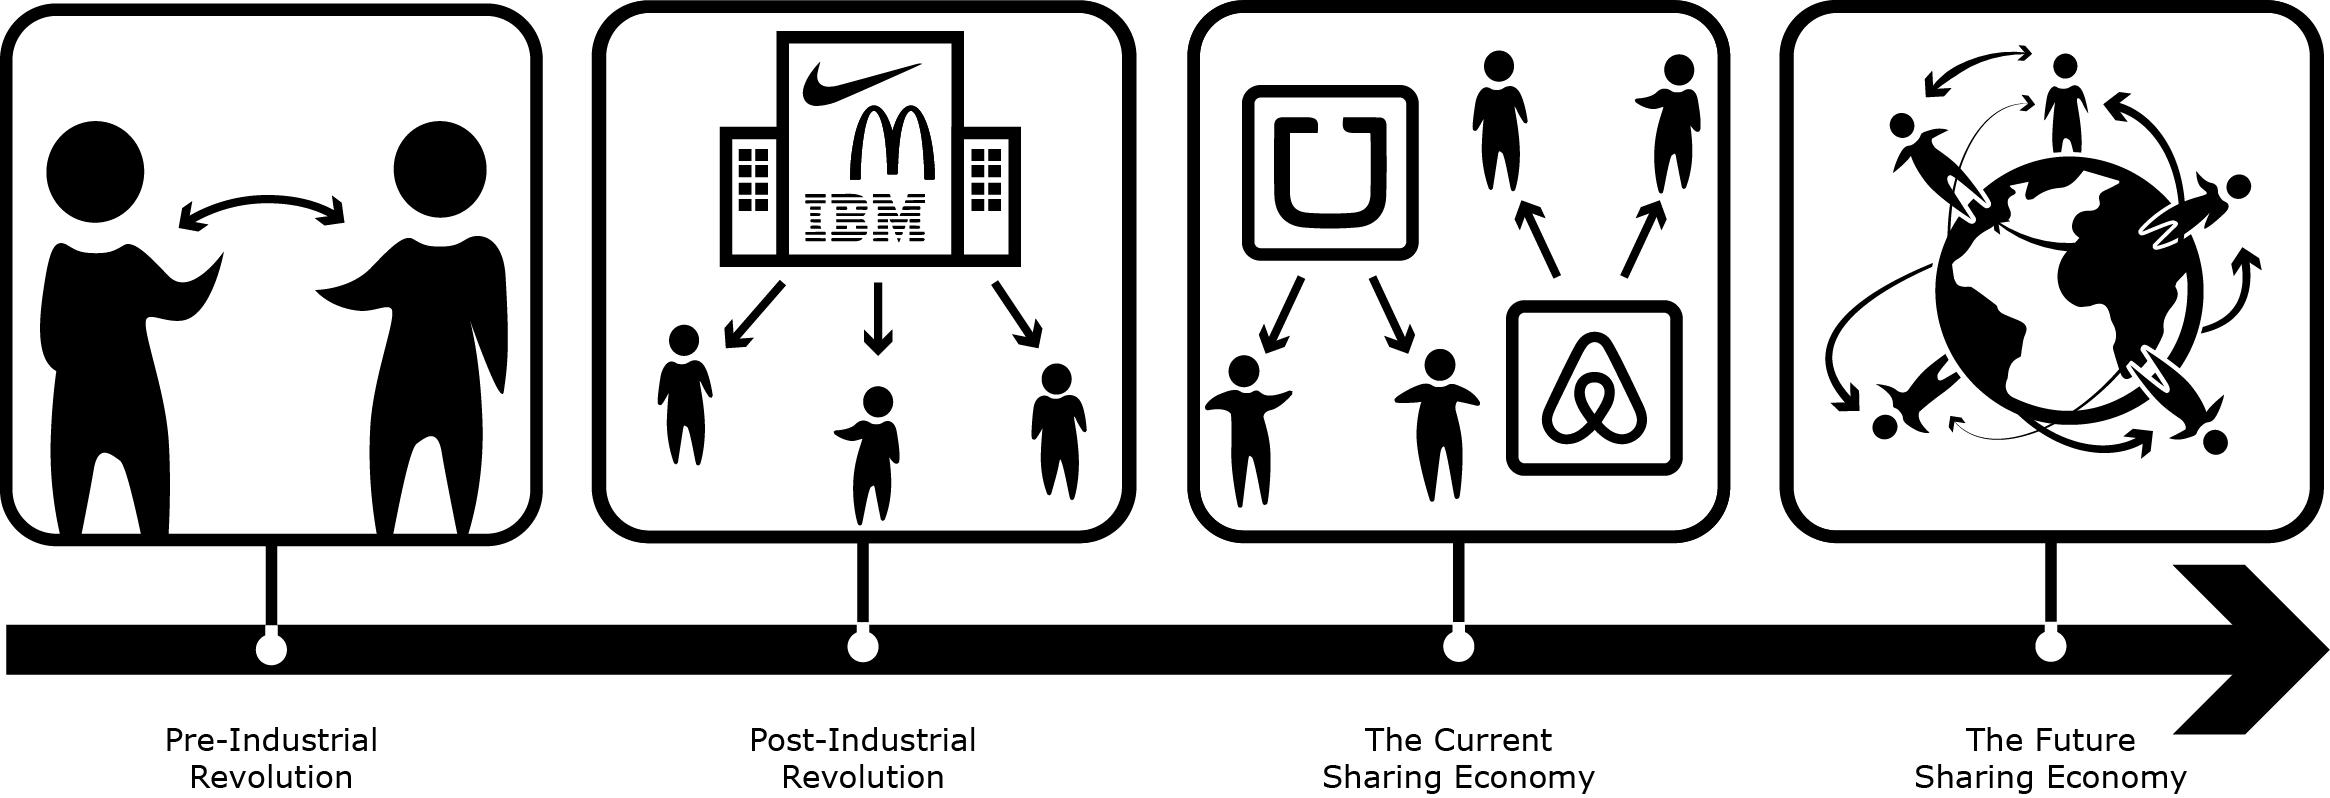
\includegraphics[width=0.8\textwidth]{images/economy.png}
    \caption{Evolution of the economy}
    \label{fig:economy}
\end{figure}

% 3. Reputation systems guide buyers towards to most trustworthy sellers on markets or help guests find houses on Airbnb that actually hold the promises made in the description. Reputation systems require three properties: dissemination, strong identities and  Yet companies take advantage of our trust and misuse our data, influence us and do not take appropriate measures to protect our data from attacks. Centralized systems are broken.
% (eBay) Ba and Pavlou, survey of reputation systems, definition of reputation system, Pouwelse 
\section{Digital trust}
{\color{red} Old: needs to be improved}
These analog, gossip-based reputation systems are what guide our decisions in buying cars, new or 
used, at which bank we store our money and at which restaurant we should have dinner.
But reputation systems are also prevalent in the digital world: we make our decisions in buying used goods 
on eBay, renting a house to a stranger (or from a stranger), getting into a stranger's car 
(what mum told us not to) based on the reputation of the partner. The sharing economy or collaborative consumption is the 
rising star of economic concepts in the information age and it is power by reputation. A company 
offers a platform on which the two sides of a trade or transaction can find each other. With each 
encounter both parties can rate that interaction and it becomes part of their history. With a longer
and more positive history the value of a profile increases as users see the reputation as security
for a good interaction and are willing to pay for it. However, there are reasons for concern. What
if the platform changes their rules in an almost unacceptable way or abuses the personal data their
users have entrusted them with? Users cannot take their reputation and data to another platform
because their reputation is actually owned by the platform facilitating the trades. Such abuses
in which trusted companies act wrongly have been happening in many times in the past, examples being
the dieselgate~\cite{VWDiesel} and the facebook/cambridge analytica scandals.~\cite{facebook} These
scandals show that even though millions of users trust them, central institutions do not necessarily
serve their customers or clients. 

% 4. The above discussion makes clear that the future digital economy requires a distributed reputation system. But making a reputation system distributed brings many additional challenges. A distributed system has no control entity which can enforce strong evidence for identities. Also single entities in a distributed system have most commonly no full view of the network, thus are not aware of all other entities or all encounters. The field is not entriely new but distributed reputation systems have been researched especially in the context of peer-to-peer file-sharing, and mobile ad-hoc system. Donation game is the game-theoretic model for this …. Although a lot of research has been conducted in the field of distributed reputation systems, major problems like the Sybil-attack, double spending, scalability and state consistency remain largely unsolved.
% Game-theoretic modeling of reputation
\section{Universal mechanism to create trust}
{\color{red} Old: needs to be improved}
We envision a future in which collaborative consumption is possible without any intermediator. This
future requires a reputation system which is application agnostic, owned by noone and ruled by 
everyone. A distributed reputation system as a layer directly
on top of the internet. However this poses some challenges from a technical
point of view. Distributed system are intrinsically hard to control and regulate, which is both 
blessing and curse. No party can impose unfair rules on other users but it is also hard to prevent 
malicious users from sending wrong information across the network. \cite{HENDRIKX2015184} reviews
state-of-the-art reputation systems and finds that all commercial reputation systems are centralized.
Some of the scientific reputation systems are decentralized like EigenTrust 
\cite{kamvar2003eigentrust}, P-Grid \cite{aberer2003p} and RateWeb \cite{malik2009rateweb}, yet
they have not been proven to work in settings where high throughput, global scaling are required 
which is the case for a global reputation system. Distributed, secure and globally scalable systems
remain an unsolved problem.

% 5. This master thesis was written in the context of the blockchain lab at TU Delft which has a long history of research on the topic of distributed reputation systems. The research is targeted at Tribler, a secure BitTorrent client which is aimed at protecting against free-riders.
% BarterCast

\section{TU Delft Blockchain Lab research}
The ambition of creating the first global trust system is realized at the Blockchain Lab of TU Delft,
which is the research group in which this thesis was created. The lab has a strong focus on exploring
new concepts, implementing them and testing them in production grade software. 

The research group has great experience and a solid track record in the field of distributed work 
systems. Especially peer-to-peer file sharing system have been studied, first and foremost the 
internally developed Tribler\footnote{https://tribler.org} application. Tribler is a client for the
BitTorrent protocol. It offers many improvements over conventional BitTorrent clients like improved
privacy and security, streaming and reputation management. It has been the testbed for algorithms of
bachelor, master and Phd students for ten years with 1 million downloads in that period. In those 
years of research several milestones have been reached. In \cite{meulpolder2009bartercast} we have 
solved the free-riding problem in the peer-to-peer file-sharing context with a reputation system 
that tracks uploads and downloads. With TrustChain \cite{OTTE2017} we have created our own 
blockchain fabric for bandwidth as a currency which builds on the previous work and adds 
tamper-proof recording and immutable history to the reputation system.

The problem of peer-to-peer file sharing systems maps well onto the trust domain. Users of BitTorrent
clients download from other users who upload data. Downloading data has benefit to users because 
they are interested in the content, however uploading has no obvious advantage. It is only necessary
to keep the content available for others. There is an obvious incentive problem, a tragedy of the 
commons. A free-rider can download without uploading, thereby consume resources without contributing.
The problem can be solved through a trust system. By recording the behavior of each user and making
it public a reputation can be assigned to each user which represents their resource usage. Users 
that contribute a lot increase their reputation while downloading decreases that reputation. Other 
users are able to inspect that past behavior of any potential partner and use it for their decision 
whether the partner deserves a contribution. 

The recording of file transactions and security of those records is facilitated by our blockchain
fabric TrustChain~\cite{OTTE2017}. TrustChain is a multi-chain fabric which lets each user create
an own chain. It is therefore built for horizontal scalability and unbounded throughput. By design,
TrustChain enables the creation of trust in any application context. The solution is implemented
in Tribler and has been used in production for more than a year as of 2018. The implementation 
details of TrustChain will be discussed more in Chapter~\ref{chap:model}. 

The great scalability of TrustChain comes at the cost of security. The architecture allows for 
attacks to be detected but the system can only be secured if honest users engage in that defensive 
behavior. This can only be ensured through incentives: agents should never be able to gain an 
advantage by circumventing the rules. 

\section{Contribution}
In this work we study a mechanism to ensure the proper dissemination and verification of transaction
records. In any trust system, the transaction records are the basis for the reputation of users and 
thus the trust users have in each other. With the records, also the reputations itself are spread, 
leading to more agreement of reputation and thus higher value. Also defending the reputation records
against attacks makes records more credible and dependable, opening applications for TrustChain with
higher requirements for security.

We will enlarge on the problem description in the next chapter. Afterwards the problem will be defined
formally and analyzed in the bounds of the definition. Before proposing a solution, some existing
approaches for recording and dissemination of data will be discussed in chapter. Next, we define a
solution based on the TU Delft blockchain fabric TrustChain and propose a specific mechanism of 
using such a fabric. Finally, we prove the correctness and scalability properties of the fabric in
experimental analysis, before concluding and making suggestions for further research.

\chapter{Problem description}
In the introduction we make a case for the decentralization of applications that handle private
information or resources and argues that scalability is one of the main problems of the promising
blockchain technology to make such systems a reality. Trustchain is an approach that removes the 
main bottleneck that restricts the scalability of the most common blockchain fabrics, namely global
consensus. However the lack of agreement on a single accepted set of transactions has many 
implications for attack resistance and correctness guarantess of the system. This chapter 
introduces these implications and defines the problem that this work is supposed to tackle.

\section{Attacks}

\subsection{Double-spend attack}
One of the most challenging attacks that exist in distributed systems is the \textit{double-spend}
attack in which an adversary creates two conflicting transactions with two different agents without
telling each about the other, effectively using resources twice. In centralized systems this attack
is prevented by the central server which processed transactions in order and realizes that the 
resources were spent in the first version of the transaction. Bitcoin was the first decentralized
accounting system that solved this problem without a central, trusted entity. However the mining
which creates a single accepted sequence for transactions is costly in terms of time and resources.
Without global consensus Trustchain (discussed in more detail in section 3) is not able to prevent 
the double-spend attack. Instead, the double-spend attack will be recorded and therefore made 
detectable. The attacker sends two conflicting transactions to two different agents and keeps one,
but both partners write the conflicting blocks on their chains. If those two agents share their 
blocks with each other or both share their blocks with a third agent, the attack becomes detectable
because the two blocks are conflicting. The prevention of this attack therefore requires 
dissemination of transaction data across the network and constant checking for conflicting 
transactions by all agents.

\subsection{Sybil attack}
During a sybil attack an adversary takes control over many entities at the same time without making
this known to the network. The attacker can then use those entities to gain influence without any
real cost because the controlled entities can create proof of transactions without actually 
performing them.

This problem is very hard to detect because controlled entities can look like real agents to 
external observers. In centralized systems this is often prevented by requiring multiple 
authentication steps, for example scanning an identity card. Also if the creation of new agents has
some costs, the adversary needs to evaluate the possible advantage against the cost of creating
multiple agents.
In Bitcoin and other proof-of-work based cryptocurrencies the attack is avoided because the power
to create a new block is proportional to computational power, so whether the computational power
is spread over multiple agents or not does not matter to the voting power in the system.

For other decentralized systems the sybil attack continues to be a challenging problem. Many 
solutions have been proposed which analyze the topology of the network. Also an initial negative 
balance has been proposed by some. Specifically for the Trustchain two algorithms, namely NetFlow
and Temporal PageRank. Yet, while the two algorithms allow for sybil-resistant calculation of a 
metric which is related to the balance of agents. Also the accuracy of the algorithms depends on 
the amount of data that is available, making it neccessary to share data between agents in order
to better be able to estimate the probability of sybils. The sybil attack will further be discussed
in chapter 4.

\subsection{Blockwithholding attack}
In decentralized systems it can be advantageous for agents to not share some information about
their transactions that would otherwise render them in a weaker position. This is not possible
in centralized systems because users do not keep their own data which instead is stored on the
central server. Thus it is not the user's decision to share or not share information with others.

In common blockchain fabrics all information is shared with everyone and only information that is 
accepted by everyone is true. By removing the global consensus this guarantee is no longer intact.
If user's own their data, they can decide to share it or not. Agents can claim that information was
lost during transactions or that a transaction did not take place.

\subsection{Dishonest behaviour}
Some application types may require agents to act according to a specific set of rules. For example
in the Tribler application, if an agent (responder) receives two requests for contribution the 
agent should contribute to the one agent that has contributed the most in the past as that agent 
deserves to be rewarded for those past contributions. Without global consensus the agent determines
the ``goodness'' of the requesters on the basis of an unobserved information set, which is a subset
of the global network information. However the agent can also decide to not stick to the rules and
contribute to the lesser of the two requesters. Without consensus on the information set on the 
basis of which the responder decides, this dishonest behaviour cannot be detected and punished by
other agents.

\section{Research question}
From the above discussion it becomes clear that removing the global consensus from any blockchain
farbics opens the system to many forms of attacks. The missing guarantees on information makes it
hard to check the correct behaviour of other agents. This makes sharing of information and 
validation of transactions an essential building block of a blockchain system without global
consensus. Yet, the question is how to enforce dissemination of transaction records without a
trusted third party. Also which information is neccessary to distribute accross the network and how
can we make sure that validation of that information is done by all nodes. Formally we can define 
the following research question:

\begin{center}
    \textit{How can we design a scalable, decentralized accounting system that ensures the distribution,
    correctness and honest usage of transaction records?}
\end{center}

The research question entails some requirements for the system that we are trying to develop. In 
the following we will explain each of those in more detail.


\subsection{Accounting system}
\label{sec:accounting_system}
The system we are trying to build is an accounting system. An accounting system keeps track of 
transactions of a resource of value between at least two parties. Accounting systems have many 
applications; two common examples are a banking system and a reputation system. Each entity in 
the accounting system has a unique identifier and from the history of the transactions recorded 
in the system a certain balance can be assigned to each identifier. When a new transaction is issued 
the balance is increased or decreased and usually some threshold is put inplace to restrict the 
infinite spending of resources. This implies that the order of transactions is of importance. As an 
example consider an entity A with the balance of 5 a minimum threshold of 0 and two transaction 
spending 4 units and 3 units two parties B and C, respectively. Obviously, it is not possible that
both transactions are accepted. Either, A first spends 4 units on the interaction with B and cannot
afford the transaction with C or the other way around. If entity A tries to submit both transactions
at the exact same time, it is the task of the accounting system to create an order of two transactions
and restrict the expenditure beyond the balance threshold.

\subsection{Scalability}
Accounting systems can exist in many different sizes and contexts, they do not even have to be
digital for some applications. However in this work we are concerned with planet-scale accounting
which even enables micro-transactions with high frequency. Therefore scalability is one of the 
main factors. Before the ascent of internet applications such dimensions were unheard of but in
the last decade services such as Facebook, WeChat or YouTube have shown that an application can 
grow to have billions of users. Our ambition is to lay the theoretical and practical basis for 
future systems that scale to these sizes. In practice that means that the transaction throughput
of the global systems needs to grow with the amount of users and that no global limit is in place
that restricts further growth.

\subsection{Decentralization}
Ownership of all transaction data can, depending on the context, give the owner power, leverage and 
value. Furthermore, a central entity creates a target for attackers and with sufficient resources
available an adversary will in the end be able to compromise the system. We see accounting systems
as a part of the infrastructure that enables applications such as banking or reputation systems. No 
single entity should be owner of such infrastructure. That is why we are considering a decentralized
solution. In the context of an internet application a centralized model assumes that one single (central)
trusted entity has access to all information and all users know and connect to that single entity. In a 
decentralized model, we cannot assume that any other entity is trustworthy or omniscent. Instead entities
are equal and communicate with each other. All users know about their own transactions and are owner of
their data, with full control over whom to share them with. 

\subsection{Distribution}
In a perfectly decentralized system each entity only knows about their own transactions. For an 
accounting system that means that each entity needs to check for themselves that they do not exceed the
balance threshold. Yet, an entity's interest could be to spend as much as possbile, which makes the 
self-control mechanism ineffective. In the context of reputation systems, an entity's interest could be
to show their good behaviour to others. In those situations a distribution mechanism needs to be put 
inplace because in a decentralized system we can no longer assume that information is simply available from
the central entity. Perfect distribution of data would mean that each user is informed about each transaction
happening on the accounting system's network. However in practice such a situation virtually impossible to 
uphold, especially when scaling to global high-frequency microtransactions. A balance needs to be found 
between the distribution of information, the scalability of the system and the storage and processing 
capabilities of each entity.

\subsection{Correctness}
In order to ensure the correctness of data multiple aspects need to be considered. First of all data needs
to be stored in a tamper-proof manner, that is, once a transaction is accepted by all parties that transaction
should not be changeable afterwards. Also the order of transactions needs to be definite, the reason for 
this was explained in Section \ref{sec:accounting_system}. Finally, entities need to be able to validate the
correctness of the state of the system.
The distribution of data informs entities in the system about the behaviour of other agents, but without
validation of that data, missing or wrong information cannot be found. This is another aspect that is often
solved by a central entity that continuously analyzes the information received by users. In a decentralized
system the validation has to be performed by each entity. For example entity A has a balance of 2 units but
is trying to spend 3 units in a transaction to entity B. Without a central entity the only party to
prevent A from transaction is entity B. B is only able to detect the invalid transaction if A has shared all
it's transactions with B and if B uses some validation precedure before engaging in a new transaction. It is
important to realize that validation is only possible if information is distributed. 

\subsection{Honest usage}
Finally, the system should make it possible to ensure the honest behaviour of entities. To show how the 
previous two components are not enough to ensure this, we can continue with the example from the previous
section. So even if B knows that the balance of A is insufficient to commit the transaction, both could 
collude and still commit the transaction. Afterwards, there is no way of knowing whether B was acting 
wrong on purpose or whether A did not share its information correctly. 

In order to ensure correct usage of the given information it needs to be possible to distinguish good from
bad behaviour. Without a central entity that knows the truth about every entity it is not straightforward to 
know which entity is the responsible one for a wrong transaction.


\section{Limitations and assumptions}

\chapter{Scalable blockchain accounting}
\label{chap:implementation}

Trust and reputation systems rely heavily on interaction records. We have shown that the problem 
of recording transactions in distributed system has been in the focus of research for many years. 
The commercial interest has lately spawned many blockchain solutions. In previous work our 
research group has deployed a blockchain-based recording system for interactions, TrustChain. This system is 
implemented in a peer-to-peer video streaming service Tribler and the IPv8 project\footnote{https://github.com/tribler/py-ipv8}. 

This chapter introduces the blockchain and the TrustChain architecture itself to the reader. We argue
that the TrustChain is a more suitable system for a trust system than a single global ledger.
Also we analyze how the TrustChain architecture can be attacked. We point
out that although detection of attacks is possible the system does not incentivize agents to share 
and verify data which is essential for the detection. In the following chapter we analyze this in the
context of a model and propose an extension afterwards. 

% Although the exchange of information is part of those systems and as shown key to their manipulation
% resistance, exchanges are not explicitly recorded. 



% % 
% % Is this necessary??? 
% \section{Reciprocity}
% % 

% \subsection{Exchanges}
% As we have shown in Chapter \ref{chap:model}, the exchange of information is a major component of a trust 
% systems defense against manipulators and free-riders. Yet, TrustChain does not create records on 
% gossip. We identify this as a limitation. 

% Honest Tribler agents actually do exchange data in order to calculate a non-zero reputation for possible
% future peers. Still, without recording of this behavior, it cannot be rewarded or its absence be punished. 
% This is why we propose an extended TrustChain which enables recording of gossip and gossip-about-gossip. 
% The details of this extension are discussed in Section \ref{sec:extension}.

\section{Blockchain basics}
The design of distributed databases bears many challenges. Especially if sensitive data is involved
and users need to have access globally, the asynchrony of events, lack of guarantees on data 
consistency and agent honesty create issues. For the early years of the internet those challenges seemed
insurmountable. That is why most services that act on sensitive data are centralized, examples being 
banks, government institutions or commercial services like Facebook\footnote{https://facebook.com}.
Centralization has its own shortcomings such as abuse of power, dishonesty, single point-of-failure
and platform lock-in. We described those issues in more detail in Chapter \ref{chap:introduction}.
The increasing significance of those issues led to the design and implementation of the Bitcoin 
protocol~\cite{nakamoto2008bitcoin} for digital money transfers. The Bitcoin protocol allows a distributed network of agents 
to agree on the exact order of events, through a hash chain which acts as a distributed timestamp 
server and the proof-of-work algorithm. This architecture is commonly referred to as blockchain or
distributed ledgers.

\subsection{Concept}
A blockchain is essentially an append-only database in the form of chained blocks. It is designed to be
used as a secure information storage in distributed systems without any central governance. 

Each block on the chain contains a set of transactions, the root hash of that set, a nonce (used in 
the consensus algorithm) and the hash of the previous block. By including a hash from the previous block,
blocks are chained together as can be seen in Figure~\ref{fig:basic_blockchain}. Any 
change to a block on the chain will change the hash of that block. This voids the following block's
hash pointer because it points to the old block. 

The first block in the chain 
is called the genesis block. The Bitcoin blockchain and similar single-chain ledgers only have 
one genesis block. Each block can also be identified by a sequence number $s \in \mathbb{Z^\geq}$, which is an increasing 
integer that starts from 0 at the genesis block.

\begin{figure}
    \centering
    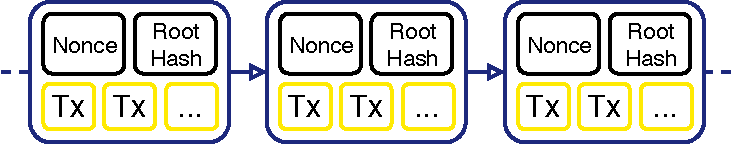
\includegraphics[width=0.7\textwidth]{images/blockchain.pdf}
    \caption{Conceptual depiction of a slice of a Bitcoin-like blockchain. Blocks contain multiple transactions and are chained together through the hash of the previous block. Source: \textit{Creation of TU Delft BLockchain Lab}}
    \label{fig:basic_blockchain}
\end{figure}

All agents are acting on the same copy of the blockchain. The one global chain therefore contains 
all transactions that happen on the network. Single global ledgers create an incentive for agents to publish new blocks by rewarding 
them with currency. New blocks are accepted if they are on top of the longest chain. This creates 
an incentive for all participating miners to stay up to date on the state of the global ledger. The
only way to create the next block and receive the block reward is acquire the latest state of the ledger.

% In order to allow for enough time to synchronize transactions and blocks, the difficulty of the puzzle 
% can be increased. This ensures a approximately fixed time between new blocks. This block time is 
% 10 minutes for Bitcoin. Together with the fixed block size the global transaction throughput of the
% system is capped. Research has shown that any proof-of-work system will not increase beyond a throughput
% of 60 transactions per second \cite{gervais2016security}. The scalability of the proof-of-work 
% algorithm is very limited which makes the Bitcoin solution only applicable in a context where high
% throughput 


\subsection{Consensus}
% why?: 
Transactions and new blocks need to be published  on the network. The block creation process
is managed by the consensus mechanism \textit{proof-of-work}. This process is also called mining and the nodes
that take part in it are thus miners. It works as follows: Each new block contains a computational 
intensive puzzle which needs to be solved in order to be able to publish a block. Specifically, 
miners are increasing the nonce $x$ until $\mathcal{H}(x) < d$ where $\mathcal{H}$ is any secure hash
function and $d$ is a target hash. The smaller $d$, the more hashes need to be calculated before finding a hash.
All miners are computing hashes until they find a correct $x$. 

Once they find a possible solution, the agent combines all the transactions that were published since the last
block and combines them to a new block. The block size is fixed such that after adding a certain number of 
transactions, the block is considered complete. If complete, the agent broadcasts the
block in the network. Any agent that receives the block will verify that
the solution to the puzzle is correct and all transactions are valid. If so, they add the new block
to their copy of the chain and start with solving the next puzzle in order to become the next 
creator of a block. 

The creator of the block is rewarded with transaction fees paid by the authors
of the included transactions and a coinbase transaction. The latter is the generation of new 
coins from a finite supply of new coins. Over time, the size of the coinbase transaction reduces 
until it reaches 0. At that point, miners are only rewarded with the transaction fees.

Conflicts can arise when two blocks are found at approximately the same time. Each block will be 
considered the latest by part of the network. The network is thus partitioned and a natural
fork is created in the chain. The conflict is resolved when the following blocks are mined. 
The partition with the larger CPU power will mine consecutive blocks faster. The longer
chain will persist as the other partition switches towards it. The mechanism ensures that (except for
the latest blocks) agents are acting on the same view of the network.

\subsection{Tamper-resistance}
% why?: show that the hash chain creates a tamper-proof record
The chain of hashes that connects blocks on the blockchain creates a theoretically tamper-proof history.  
Changes to any block will alter its hash and break the chain of hashes. Therefore any change to the 
block requires the recalculation of all following blocks. Because all blocks need to be agreed upon on the network 
other agents will be able to see such tampering with the blocks and will not agree on it. 

Similarly the order of blocks is ensured through the hash pointers. Any change to the order of blocks
will will result in a break in the hash chain.
The sequence of blocks also orders the transactions stored in the blocks. 
Any transactions in an earlier block happen before the transactions in the later block. Also, as was just 
explained, any change to the ordering of transactions. Even though this order
does not necessarily correspond to the local time of the agent who published the transaction, the 
blockchain will create a globally accepted order for transactions.  This is a major 
achievement because this order is robust against network delays, tampering and other attacks.

However, proof-of-work blockchain are not truly tamper-proof. The tamper-resistance is ensured through
mining power. As long as more than 50\% of the network's CPU power is controlled by honest agents, 
the correctness of the system is ensured. However, if any attacker is able to obtain a majority of
computing power, any tampering can be possible because the attacker can mine invalid blocks faster
then the honest minority. For very large networks such as the Bitcoin network, the probability of 
a single attacker having a majority of CPU power is very small. However, smaller networks or collusion
attacks in which multiple miners work together can be successful as shown by some examples~\cite{51percentbitcoingold, 51percentverge}.

The majority of the mining power can also be used to create a intentional fork in the chain in order 
to fix software bugs. If a majority of miners update their software to version that creates and verifies blocks
differently while a minority continues with the old software, a hard fork is created such that two
version of the blockchain are continued. Examples of this are Bitcoin Gold \footnote{https://bitcoingold.org} and Ethereum Classic \footnote{https://ethereumclassic.org}.

\subsection{Scalability}
A single global ledger like Bitcoin seems like a valid implementation for recording transactions for a
trust system. All transactions are exchanged with all agents on the network. The blockchain 
creates a totally ordered set of all global transactions which intrinsically means that each agent's 
transactions are also fully ordered. Double spend and forks are detectable through global consensus. 

However, the proof-of-work mechanism leads to issues in scalability. It restricts the global throughput
to at best 60 transactions per second~\cite{gervais2016security}. This is not enough to power a global-scale distributed trust 
system as we envision it. The proof-of-work consensus algorithm also leads a to a large expenditure of energy which creates 
large transaction costs. This is not acceptable if the trust system should be for general purpose 
applications. For example, users will not accept to pay for each video they stream on the Tribler 
platform. A different solution is therefore needed.

In Section \ref{sec:related_work} several improvements to the scalability are mentioned. Examples are
alternative consensus protocol such as proof-of-stake and delegated proof-of-stake. Also, sharding
and off-chain transaction channels have been proposed which are supposed to increase throughput.
Each solution balances three design variables: decentralization, scalability and consistency. This
is commonly called the scalability trilemma in blockchain communities \footnote{For example mentioned in the Ethereum wiki. https://github.com/ethereum/wiki/wiki/Sharding-FAQs}.
Crytpocurrencies generally target decentralization and consistency as the driving design factors. 
Financial transactions have high value and require consistency. Secure payments are enabled while 
scalability is less important.


\section{TrustChain}
\label{sec:trustchain}


TrustChain's design focus is in stark contrast with that of
Bitcoin. Instead of employing global consensus to guarantee a single global ledger, 
all agents in the TrustChain fabric are owner of a chain for themselves. This creates a scalable 
solution in which the total network throughput grows with the size of the network. However, the
scalability comes at the cost of consistency guarantees. 

We argue that when designing a global-scale
trust system, interaction throughput has higher value than consistency. Although undesired, we 
consider the manipulation of an agents reputation as less severe than stealing large amounts of 
money. Therefore, an architecture such as TrustChain with unbounded scalability is a better basis
for a trust system than single global ledgers.

We continue this chapter with a description of the TrustChain architecture.

\begin{figure}
    \centering
    \begin{subfigure}{0.49\textwidth}
        \centering
        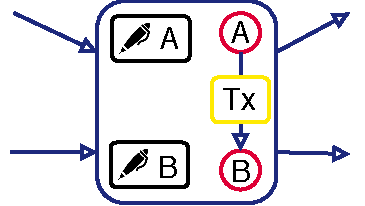
\includegraphics[width=0.8\textwidth]{images/block-2.pdf}
        \caption{Conceptual representation}
    \end{subfigure}
    \begin{subfigure}{0.49\textwidth}
        \centering
        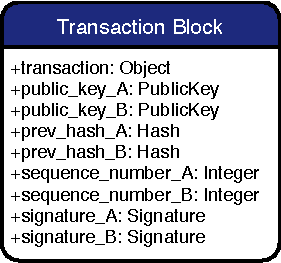
\includegraphics[width=0.6\textwidth]{images/transaction_block_data.pdf}
        \caption{Transaction block, data representation}
    \end{subfigure}
    \caption{A single block in the TrustChain fabric. Incoming arrows represent block hashes from the previous blocks of the agents' chains. Source: \textit{Creation of TU Delft BLockchain Lab}}
    \label{fig:trustchain_block}
\end{figure}

\subsection{Data structure}
\label{sec:transaction_blocks}
Similar to the Blockchain architecture TrustChain records transactions in blocks and links blocks 
with the use of hash pointers. Though, in contrast to having a single chain of blocks for the whole
network, in TrustChain each agent starts with an own genesis block. Hence, all agents record their
own transactions on their chain. 

Blocks in TrustChain contain exactly one transaction between two parties. Because both parties have 
their own chain and the transaction concerns both parties, any new block is added to both agents'
chains. Each block contains the following main elements:

\begin{itemize}
    \item \textbf{Transaction.} The transaction field records the value that was exchanged between agents.
    TrustChain is designed to be application agnostic. Thus the content of a transaction can be any 
    serializable data. 
    \item \textbf{Previous block hashes.} The hashes of the previous blocks of both agents' chains 
    firmly attaches the new block to their history. This is similar to the basic blockchain concept.
    \item \textbf{Public keys.} In order to uniquely identify the two agents that conduct a transaction
    their public keys are recorded.
    \item \textbf{Signatures.} Both agents provide a digital signature of the transaction with their 
    private key which any agent can check with the agents' public keys. This authenticates the 
    transaction and cryptographically proves that the real owners of the private key conducted the 
    transactions.
    \item \textbf{Sequence numbers.} All blocks on an agent's chain have a unique sequence number 
    which shows the position in the chain. 
\end{itemize}

A simplified depiction and data representation of a TrustChain block is shown in Figure~\ref{fig:trustchain_block}. When 
looking at a single agent the given data structure creates a chain of blocks which describes all the
transactions of that agent. However the second incoming and outgoing edge of each block entangles an
agent's chain with those of all partners. When looking at a complete network, of the transactions the
represents a directed acyclic graph(DAG). Such a structure is shown in Figure~\ref{fig:trustchain_graph}.

\begin{figure}
    \centering
    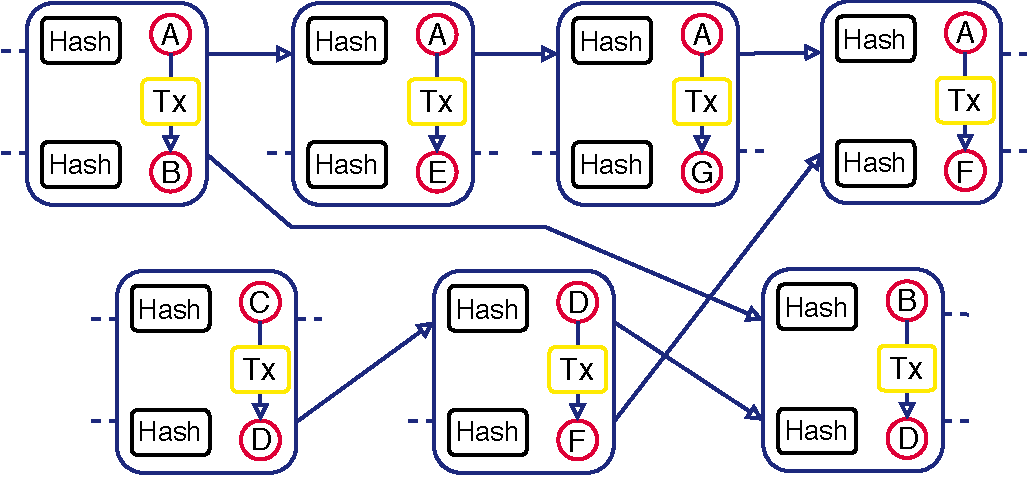
\includegraphics[width=\textwidth]{images/trustchain_graph.pdf}
    \caption{TrustChain graph structure with multiple transactions. The top row shows the chain of
    an agent A with links to multiple other blocks. Source: \textit{Creation of TU Delft BLockchain Lab}}
    \label{fig:trustchain_graph}
\end{figure}


\subsection{Verification protocol}
\label{sec:validation}
TrustChain blocks are designed in a way to be verified by any other node. The verification is 
required to ensure that the block has not been tampered with and is correctly connected to a valid 
chain. A block can only be valid if all of the following conditions are true:

\begin{enumerate}
    \item The transaction field contains the necessary information to properly define a transaction 
    in the application context. For Tribler it needs to contain at least the amount of data which 
    was uploaded and downloaded between the two agents. 
    \item Both block hashes need to point to the valid, previous block on the chain of the same 
    public key. This makes the validity a recursive definition which depends on the previous content
    of the chain of both agents.
    \item Both public keys need to be valid public keys.
    \item The signatures need to be correct for the given public keys and block content.
    \item The block needs to carry the next integer as sequence number compared to the blocks that 
    the previous hashes point to.
\end{enumerate}

The true validity of a block can only be established if the verifier also checks all other blocks on
the chains of both parties. Yet, that implies to check all other blocks of their partners and their
partners. Such a strong form of validity can thus only be ensured by verifying an exponentially 
growing amount of blocks.
% A block can only be valid if the hash pointers also point at valid blocks. This recursive definition
% requires agents to either verify the complete chain of both agents up to the block to be verified or
% assume that all previous partners have also verified their transactions. 

A weaker form of validity can be that the previous blocks pointed at, exist. That does not ensure 
the validity of the complete chain but allows for a simple non-recursive validity check.

\subsection{Tamper-evidence}
\label{sec:tamper-proof}
Blocks of the TrustChain architecture are tamper-evident. Blocks are chained through hashes of their
content and signed by both transaction parties. Any change to the content of the block, that is the
transaction field, the sequence numbers, the signatures, previous hashes or public keys will change
the hash of the block. Also, any such change will invalidate the original signatures of both agents. An agent
can renew her own signature but not the signature of the partner without access to the 
partner's private key. Apart from the invalid signatures also any consecutive block's previous hash
will be invalid because the tampered block's hash has changed.

We can conclude that any tampering of a block will be evident to an agent that performs verification
of the signatures and hash pointers of consecutive blocks.

\subsection{Scalability}
\label{sec:trustchain_scalability}
For a transaction to be successful in TrustChain, only the involved agents need to agree on the content. This
means that only two agents need to communicate to confirm a transaction. Transactions do not need to 
be publicly announced or sent to all nodes on
the network. Also, multiple transactions can be performed at the same time globally without breaking
the rules of the system. In contrast to the Bitcoin system, only the transactions of each agent are
strictly ordered, the global set of transactions is not.

This results in a system that scales with the size of the network. A simple example makes this very 
clear. Consider two networks, one with 10 nodes and one with 100 nodes. For simplicity we consider
time to be discrete and agents to interact in rounds. Each transaction takes 1 round and all agents 
interact. Throughput calculation is then straightforward. Nodes arrange in pairs and perform a
transaction. The small network will have 5 pairs and thus 5 transactions per round, while the large
network has 50 pairs and transactions. Although this example is extremely simplified, no real-world
effect like network delays, network churn or bandwidth restrictions greatly conflict with this property.

TrustChain does not include a global consensus and thus does not expend bandwidth, storage and 
computational power to create a global order for transactions. That removes the most costly component
from the general blockchain architecture. Without the expense of CPU power to calculate hashes as in the proof-of-work mechanism,
transactions only cost the bandwidth and computational expense of communicating with 
the direct interaction partners. TrustChain enables free transactions in a global distributed 
system with scaling throughput based on the network size. Hence, TrustChain is valid solution for a
global trust system.

\subsection{Security}
The superior scalability of the TrustChain architecture compared to single global ledgers comes at 
the expense of some security guarantees.

Similar to a single Blockchain the graph structure of TrustChain creates a tamper-proof record of
transactions. A large difference is that each agent reigns over a chain. Each agent seemingly is 
able to reorder transactions but blocks are signed by a second agent and the signature will become
invalid if the blocks are tampered with. Also blocks contain the previous hash of the counter party's
previous block. That ensures that the hashes cannot change without the other agent being able to 
detect the tampering.Therefore transactions are still recorded in a tamper-proof data structure.

Still, detectabillity does not ensure detection. The can only be secured if agents
continuously verify their partners data. Also, as the validity of a block is recursively defined, 
agents can only ensure the validity of a partners previous transaction if they possess their complete
chain and verified that chain. It is even harder to defend against attacks in which agent do not 
directly manipulate the data structure but make use of the incomplete knowledge which is intrinsic 
to distributed networks. 

% A prominent example, the double spend attack, has been defined and extensively 
% discussed in Chapter~\ref{chap:model}. We have shown that gossiping, that is sharing of knowledge, 
% is a way to detect such attacks. The current
% TrustChain system does not record gossiping in any way. Therefore agents do not have a strong 
% incentive to perform gossiping. In the next section an extension will be discussed which adds the 
% possibility of recording exchanges.

\section{Security analysis}
\label{sec:attacks}
If the trust system works as expected, a good reputation should have value to agents. All agents on 
the network attempt to obtain a good reputation and be seen as a trusted partner. As such their 
behavior should be meticulously agree with the rules. Yet, if the value is large enough and behaving
well comes at a large enough cost, agents will aim to bend the rules or even break them in a smart 
way in order to get the good reputation for free. As a designer of the trust system it is essential
to predict the possible ways of manipulation and prevent them. In this section we will define several
known types of attacks on trust systems and if applicable define how TrustChain can prevent them.

\subsection{Block manipulation}
\label{sec:tampering}
Block manipulation has been introduced previously. An agent changes a property of a block in his 
chain, distorting the true history in order to gain an advantage. For example, a block records a 
transaction in Tribler in which agent $A$ downloaded from agent $B$. The transaction reduces the 
reputation of agent $A$ which is why $A$ could decide to change the amount of data downloaded to 0.
If agent $A$ does this before the signatures are provided, $B$ will not agree to sign the transaction
and will ignore $A$ in the future because $A$ obviously is not an honest partner. On the other hand,
if both agents sign the transaction first, $A$ can change the value on his own chain without $B$ 
immediately noticing. The signature of $B$ however becomes invalid because $B$ signed the original, 
correct version of the block. In any following transaction, any agent $C$ that is about to interact
with $A$ has the chance to detect this fraud by checking the signatures on all previous transactions
of $A$. 

TrustChain makes any manipulation detectable. Still if agent $C$ collaborates with agent $A$ or 
agent $C$ is ``lazy'' and does not obtain $A$'s chain to verify it prior to an interaction, $C$ can 
perform a transaction. The collusion or laziness cannot be detected and $C$ will remain honest 
in the eyes of future partners.

\subsection{Forking and double-spending}
Forking is one of the most well-known attacks of blockchain based systems. In the cryptocurrency 
context it is also known as double spending. An attacking agent 
performs two conflicting transactions with two different partners. This translates to two transaction
blocks which have the same sequence number for an attacking agent $A$. Partner $B$ and $C$ are each
not aware of the other version of the block and will sign the block. This allows to ``overwrite''
a negative transaction (with $B$) with a positive transaction (with $C$). $A$ will only keep the positive transaction on 
the chain. 

TrustChain makes this attack detectable through the sequence number of the blocks. If any agent 
obtains both versions of the block, that agent will see that $A$ has signed and thus authorized the
creation of two blocks with the same sequence number. Also if $B$ obtains any later blocks from $A$ 
the hashes will not point to the transaction with $B$.  This creates a \textit{proof-of-fraud}. 

The actual
detection of this attack requires agents to obtain transactions from their peers and compare those 
to existing blocks. Because no agent is aware of the transaction with $B$, agents cannot not specifically 
request $B$'s history to check for the attack. Therefore, the detection requires the collaboration
of the network in the form of random block requests. As we will show in Chapter \ref{chap:model}, 
without exchanging information about their transactions, agents are not able to find a double-spender.

\subsection{Block withholding}
Once agents have a longer history they will have records of positive and negative encounters. A 
malicious agent then might try to hide any records of negative encounters, thus boosting the trust 
others have in the attacker. The architecture of TrustChain makes such an attack easily detectable.
The blockchain of any agent creates a tamper-proof, irreversible order for all transactions. Only if
the sequence numbers increase exactly by one to each following block can another agent be sure that 
the whole history was shared by an agent. Therefore to establish the trustworthiness of an agent, 
another agent at least needs to obtain their full chain.

Note that if an agent witholds the latest blocks, this cannot be detected by another agent (except
if that information was obtained already through gossiping). Yet such an attack is similar to a
double-spend because any newly created block will conflict with those blocks that were withheld.

\subsection{Whitewashing}
Agents that have a significantly bad reputation such that finding interaction partners becomes difficult may decide to create a new 
identity for themselves. Thus, they can rid themselves from the bad reputation and start fresh. This 
type of attack is called whitewashing. In the currently deployed version of TrustChain in Tribler 
this attack cannot be prevented as the software is free and new agents do not need registering with
any central institutions.

Still the impact of such attacks can be limited by having some mistrust of new agents joining the 
network. In that case new agents need to ``pay their dues'' before being accepted by the network 
as equals. For example, assume honest agents only upload data to agents that are above a certain level
of reputation. Once an agent is below that boundary he needs to upload data before downloading again.
Also, new agents start at that boundary level of reputation. In that case whitewashing will not be
possible. However the question then remains how the system can be bootstrapped and maintained
active because with each new agent the overall network reputation decreases such that at some point
only uploading is possible but no agent is able to download.

\subsection{Sybil attack}
One of the most serious attacks on trust systems is the Sybil attack. In a Sybil attack, the attacker
creates a set of new fake agents, called the Sybils. Together with the attacking agent the set of 
agents is called a Sybil region in the network. The Sybils create transaction blocks  
between each other without actually performing the transactions with the goal of boosting the 
reputation of one of the agents in the Sybil region. The attack is successful as honest agents 
cannot distinguish between fake and real transaction records. Each Sybil has a valid public and private
key and is able to sign transaction blocks. They create valid transaction data without any neccessary
manipulation or proof-of-fraud.

Multiple ways have been explored to prevent this attack. One way is to analyze the network topology
and use it to detect Sybil regions. A trust mechanism such as NetFlow, which has been proposed in 
\cite{OTTE2017} is resistant against weakly beneficial Sybil attacks. Another way is to increase the cost of 
registering new identities in the system. If each registered public key needs to be anchored on a 
costly blockchain like Bitcoin, it becomes much harder to create a Sybil region. We leave this problem
to future research.

\subsection{Collusion}
\label{sec:collusion}
Attacks are called a collusion attack if multiple attackers work together to achieve a beneficial
situation for at least one of the colluders. Attacks such as those described above, 
can become more successful when multiple attacks collude. An example of this was given for block 
manipulation. If one agent manipulates a block and afterwards interacts with a colluder to share the
wrongly obtained positive reputation, the colluders chain seems completely valid to honest agents.

In TrustChain it is hard to detect such collusion because we do not know whether agents actually 
did not know about an attacker or just claim so. We will next look at an extended system which 
records the knowledge of agents. Although this creates protection against some collusion attacks, 
still not every collusion can be protected against.

\section{Chapter conclusion}
TrustChain is a scalable solution for tamper-evident recording of transactions in a distributed 
network. It therefore fulfills many of the requirements that we set for our system in the previous
chapter. However, TrustChain cannot in itself provide consistency of interactions as we have shown
with the discussion of the double-spend attack. We show in the next chapter that gossiping is a
valid solution to solve this problem. Still TrustChain provides no strong incentive for agents to 
gather blocks from their peers. This opens the system to free-riders who do not exchange information and verify 
blocks but remain honest in the eyes of their peers. 

Additionally, the lack of incentive for gossiping decreases the probability of indirect reciprocity
because agents are not aware of each others good or bad reputation.
As we have discussed in the previous chapter, global-scale trust system will mostly rely of indirect
reciprocity. Therefore the dissemination of data is essential to our system.

On the other hand, such a strong exchange policy leads to a challenging storage and bandwidth 
requirement. Each agent's subjective network state will approximate the complete networks data.

\chapter{Formal model}
\label{chap:model}
We aim to show the importance of dissemination and verification of interactions 
records. This is done by defining a model within which we can prove with rigorous math that record
dissemination and verification are essential for securing the trust system. Also we define a
mechanism which allows to protect the network against free-riders which 
jeopardize the overall security. Our proposal is to introduce gossip transparency which can 
effectively punish free-riders that do not acquire and disseminate interaction records. We further 
show that it is possible to detect agents that consciously interact with malicious agents, exposing
them as verification free-riders or accomplice.

\section{Model definition}
\label{sec:definitions}
We make use of the ordered interaction model which has been introduced in previous work from 
our research group by Otte et. al. in \cite{OTTE2017}. We restate it in Definition \ref{def:old_base} for clarity.
The symbols were annotated in order to reuse symbols in later definitions.

\begin{defn}[Ordered interaction model]. 
    \label{def:old_base}
    An ordered interaction model $\hat M = \langle \hat P, \hat I, \hat a, \hat w \rangle$ consists of two sets and two 
    functions.
    \begin{itemize}
        \item $\hat P$, a finite set of agents
        \item $\hat I$, a finite set of interactions
        \item $\hat a : I \rightarrow P \times P$, a function mapping each interaction to the agents 
        involved in it.
        \item $\hat w : I \times P \rightarrow \mathbb{R}_{\geq0}$, a function which describes the 
        contribution of an agent in an interaction
    \end{itemize}
\end{defn}

The model allows for the analysis of any type of application in which a network of agents performs
transactions that can be described by a quantitative amount. However, the model does not explicitly
model the information exchange between agents. Our goal is to show that in a distributed trust system this 
exchange of information is also an essential component to guarantee manipulation resistance. We 
therefore extend the model with this concept of exchange.

\begin{defn}[Ordered encounter model]. 
    \label{def:base}
    An ordered encounter model $M = \langle P, I, E, a, w, x \rangle$ is a 6-tuple consisting
     of three sets and three functions. For convenience we define a set $N = I \cup E$. 
    \begin{itemize}
        \item $P$, a finite set of agents
        \item $I$, a finite set of interactions
        \item $E$, a finite set of exchanges
        \item $a : N \rightarrow P \times P$, a function mapping each interaction to the agents 
        involved in it.
        \item $w : I \times P \rightarrow \mathbb{R}_{\geq0}$, a function which describes the 
        contribution of an agent in an interaction
        \item $x : E \times P \rightarrow N^+$, a function which describes the interactions that an 
        agent received in an exchange. $+$ refers to the Kleene plus.
    \end{itemize}
\end{defn}

We call the set $N$ the encounters of the model. An encounter happens between two agents for one of
two reasons: to perform a transaction of some value or to exchange information.
Interaction in this model are the equivalent of transactions of value in an application context. 
An exchange on the other hand is a transaction of information about other encounters.
The function $x$ describes a set of encounters that an agent obtains through an 
exchange. The process of exchanging data is also called gossiping. We will formally introduce the 
knowledge concept in Definition~\ref{def:subjective_network_state}.

For each agent we can describe the set of encounters which that agent participated in as the agent 
encounter history. 

\begin{defn}[Agent encounter history]
    Given an ordered encounter model $M = \langle P, I, E, a, w, x \rangle$ the agent encounter history of an agent $p \in P$ is defined as follows:
    \begin{equation}
        H_p = \{ n \in N : p \in a(n) \}
    \end{equation}
\end{defn}


The history of an agent $p$ is totally ordered by $<$. If we denote the 
$t$th encounter of $p$ as $n_p(t)$ then we can alternatively write $N_p = \{ n_p(1), n_p(2), ..., n_p(i)\}$.
This notation will be handy in a later definition.

Encounters between agents are not public. This creates a discrepancy between the true set of 
encounters $N$ and the observed encounters from an agent $p$'s point of view. Agents only have 
knowledge of those encounters which they participated in or which they obtained knowledge of through an exchange.
We can then define the subjective network state, which is the knowledge an agent has about the state of
the network.

\begin{defn}[Subjective network state]
    \label{def:subjective_network_state}
    Given an ordered encounter model $M = \langle P, I, E, a, w, x \rangle$ and an agent $p \in P$ with encounter history $H_p$, the subjective network state of agent $p$
    is defined as follows:
    \begin{equation}
        N_p = \{ n \in N : n \in H_p \} \cup \{ x(e, p) : e \in E \}
    \end{equation}
\end{defn}

The subjective network state contains the complete knowledge of the agent. In \cite{OTTE2017} a 
similar concept exists in the form of the subjective work graph. It generally models a partial view
of the network described by the model. This subjective view is the basis for the calculation of 
reputation and trust as further described by Otte et.al.. At the core of this work is not the way 
reputation and trust are calculated but rather how the knowledge of interactions is disseminated and
protected against malicious agents. The relation to actual trust creation is further discussed in 
Section \ref{sec:relevance}

The model from Definition \ref{def:base} introduces the concept of exchanges. Yet it does not define
how agents should exchange data. We therefore define an exchange policy which is the strategy that 
honest agents apply for exchanging information.

\begin{defn}[Exchange policy]
    Given an ordered encounter model $M = \langle P, I, E, a, w, x \rangle$ and an agent $p \in P$ with encounter history $N_p$,
    the exchange policy is a function $f : I_p \rightarrow P \times N^+$, where $I_p = \{ n \in N_p  \cap I\}$.
    The exchange policy maps each interaction of an agent $p$ to a partner and set of encounters 
    which need to be obtained from that partner prior to the interaction.
\end{defn}

The exchange policy defines which information an agent needs to have in order for an interaction to 
be valid. This is to ensure that an agent has all the information to ensure that the partner is also
an honest agent. It should be noted that an honest agent has no reason not to reply to an exchange 
request. 

As the exchanges are recorded it is possible to determine whether an agent adheres to a certain 
exchange policy. 

\begin{defn}[Exchange policy adherence]
    Given an ordered encounter model $M = \langle P, I, E, a, w, x \rangle$ and the history $H_p$ of an
    agent $p$, the condition for adhering to a policy $f$ and
    therefore being considered an honest agent is as follows: 

    \begin{equation}
        f(I_p) \subseteq \{ (q, x(e, p)) : e \in H_p \cap \in E,  \exists (p, q) \in a(e)\}
    \end{equation}
\end{defn}

% The subjective network state also implies the known agents $P_p = \{ q \in P : n \in N_p, q \in a(n) \}$
% Without full observability there is also no guarantee that agents know the full history of their 
% peers. Actually the subjective network state defines also $p$'s observed peer history of an agent $q$.

% \begin{equation}
%     H_{p, q} = \{ n \in N_p : q \in a(n) \}
% \end{equation}

% Similar the observed peer history is a totally ordered set. It is not necessarily equal to the 
% complete history though. For example, an agent $q$'s history $H_{q} = \{n_q(1), n_q(2), n_q(3) \}$
% could be observed by an agent $p$ as $H_{p, q} = \{n_q(1), n_q(3)\}$.

% Finally, a reputation mechanism needs to be defined. Agents estimate the reputation of their peers
% from their subjective network state. 

% \begin{defn}[Reputation mechanism] 
%     A reputation function $R$ takes as input the subjective network state $N_{p}$ and determines 
%     a reputation score $S^R_{p,q}(I_{p,q}) \in \mathbb{R}$ for all known agents $P_p$.
% \end{defn}

\section{Fork and double spend defense}
\label{sec:model_double_spend}
In what follows we analyze the impact and defense of the previously defined model against a double spend attack. That is a potent 
attack on a network that can be modelled by an ordered encounter model. Conceptually, an attacker 
has two conflicting interactions at the same time with two different agents. As each partner is not
aware of the other both accept the interaction. 

\begin{defn}[Fork and double spend]. Given an ordered encounter model $M = \langle P, I, E, a, w, x \rangle$, a malicious agent $p$ has two conflicting interactions 
    $i \in I$ and $j \in I$ at the exact same time. Both interactions have a different partner $a(i) = (p, q)$ 
    and $a(j) = (p, r)$ Accordingly, the personal history  of $p$ is not a totally ordered set anymore.
    The attack can be detected if for any honest agent $s$, $i_p(t) \in N_{s}$ and $i_p(t)' \in N_{s}$ are
    true.
\end{defn}

In the following we show that gossiping is essential for the network to defend against such an 
attack. We first study the case of no exchanges. For that we formally define the No-Exchange policy.

\begin{pol}[No-Exchange]
    \label{pol:no-exchange}
    The No-Exchange policy defines no required exchanges for an honest agent, so $f(I_p) := \emptyset$.
\end{pol}


\begin{thm}[Detectability of double spend without gossiping]
    \label{thm:fork_no_gossiping}
    If honest agents apply the No-Exchange policy, and therefore do not perform gossiping,
    the fork and double spend attack cannot be detected.
\end{thm}
\begin{proof}
    Let $p$ be the attacking agent and let $i$ and $j$ be the conflicting interactions of the 
    attacks. Further, let $q$ be the partner in interactions $i$ such that $a(i) = (p, q)$ and let 
    $r$ be the partner of interaction $j$ such that $a(j) = (p, r)$. 
    No gossiping implies no exchanges $E = \emptyset$ and therefore for any agent $s$ $N_s = H_s$
    applies. 
    According to Definition \ref{def:subjective_network_state} $i \in N_{q}, j \notin N_{q}$ and 
    $i \notin N_{r}, j \in N_{r}$. Without gossiping both $q$ and $r$ will not further disseminate 
    their interactions with $p$ and therefore will not learn of the other version.
    Moreover, all other agents $s \in P$ are aware of neither $i$ or $j$ because only direct 
    interactions are observed. Consequently no agent observes both $i$ and $j$.
\end{proof}

Theorem \ref{thm:fork_no_gossiping} proves that without gossiping the double spend attack cannot be
detected without gossiping. We now show that gossiping can lead to the detection of the attacker. We
define an exchange policy in which honest agents obtain the encounter history prior to an interaction.

\begin{pol}[History-Exchange policy]
    \label{pol:one}
    The History-Exchange policy requires agents to obtain the encounter history of their partner 
    prior to an interaction. 

    \[ f(I_p) := \{ (q, H_q) : \exists i, q (i \in I_p \text{ and } (p, q) \in a(i)) \}\]
\end{pol}


\begin{thm}[Detectability of double spend with gossiping]
    \label{thm:fork_gossiping}
    If all honest agents apply the History-Exchange policy and periodically use uniform sampling over
    the set of agents to find an interaction partner, the double spending will eventually be detected.
\end{thm}
\begin{proof}
    Let $p$ be the attacking agent and let $i \in I$ and $j \in I$ be the conflicting interactions 
    of the attack at time $t$. Further, let $q$ be the partner in interactions $i$ such that 
    $a(i) = \{p, q\}$ and let $r$ be the partner of interaction $j$ such that $a(j) = \{p, r\}$. 
    According to Definition \ref{def:subjective_network_state} $i \in N_{q}, j \notin N_{q}$ and 
    $i \notin N_{r}, j \in N_{r}$.

    We consider an honest agent $q$ sampling agents for an interaction. For network size $l = |P|$ the 
    probability of choosing partner $r$ in the first round is $1/l$. The probability for not having
    chosen $r$ in any of $k$ rounds is $(\frac{l-1}{l})^k$ and $\lim_{k\to\infty}(\frac{l-1}{l})^k = 0$.
    At some point $q$ therefore choses $r$ for an interaction and because $q$ is honest performs an 
    exchange $e$ prior. $j \in H_r$ and therefore $j \in x(e, q)$, which means that after exchange 
    $e$ $i \in N_q \text{ and } j \in N_q$. Therefore $q$ is able to detect the double spending.
\end{proof}

Theorem \ref{thm:fork_gossiping} shows that gossiping makes double spending detectable. Once a double
spender is detected by an agent it is possible to ignore them for future interactions. The amount 
of exchange rounds until detection depends on the exact policy of exchanging data and a deeper 
analysis is beyond the scope of this work.

\section{Gossip free-riding}
Our aim is now to show that a reputation mechanism which takes into account the exchange behavior of 
agents defends the system against gossiping free-riders. 

If bandwidth and storage capacity are valuable resources for agents, data dissemination and their 
long-term storage come at a cost for agents. Therefore agents can attempt to free-ride and only 
interact without exchanging data. However if all agents would behave in that way the system loses 
the ability to defend itself against forks and double spending as shown in Theorem 
\ref{thm:fork_no_gossiping}. We will call those agents gossiping free-riders. 

% An honest agent should also be able to verify that other agents adhere to an exchange policy or not.

% \begin{lem}[Exchange policy adherence]
%     \label{lem:policy_adherence}
%     Given an ordered encounter model $M$ with exchange policy $D$, any agent $p$ that has observed 
%     the complete history $H_s$ of an agent $s$ can determine whether that agent adhered to policy 
%     $D$.
% \end{lem}
% \begin{proof}
%     Agent $p$ has observed the complete history of agent $q$, therefore $H_q \subseteq N_p$. Agent 
%     $p$ is then able to calculate the frequency of $q$'s exchanges as $f^D_q = \frac{|\{ n \in H_q : n \in E \}|}{|\{ n \in H_q : n \in I \}|}$,
%     the partners of exchanges $S^D_q = \{ a(n) \setminus q : n \in H_q \text{and} n \in E \}$ and the 
%     exchanged encounter $E^D_q = \{ x(n,q) : n \in H_q \text{and} n \in E \}$. Then $p$ can compare
%     the calculated values to the expected values defined by $D$. 
% \end{proof}

\begin{defn}[Gossiping free-rider]
    \label{def:gos_free-rider}
    Given an ordered encounter model $M = \langle P, I, E, a, w, x \rangle$ with exchange policy $f$, a gossiping free-rider $p \in P$ is an 
    agent whose exchange behavior does not fulfill the minimum requirements of policy $f$. That is, 
    $f(I_p) \nsubset \{ (q, x(e, p)) : e \in H_p \cap E, \exists (p, q) \in a(e)\}$.
\end{defn}

We now show that gossiping free-riders can be detected by honest agents that apply the History-exchange
policy.

\begin{thm}[Detectability of gossiping free-riders]
    \label{thm:gos_free-rider}
    Given an ordered encounter model $M = \langle P, I, E, a, w, x \rangle$ in which honest agents use the History-Exchange policy
    a gossiping free-rider can be detected on the first interaction.
\end{thm}
\begin{proof}
    Assume agent $p$ is an honest agent and is about to interact with agent $q$. Because agent $p$
    uses Policy \ref{pol:one}, $p$ will request an exchange with $q$. That exchange will contain 
    $H_q$. If it does not $p$ will know that $q$ is a gossiping free-rider. After a successful
    exchange $H_q \subseteq N_p$. In that case $p$ is able to check the condition for adherence to 
    the History-Exchange policy $f$ by $f(I_q) \subseteq \{ (q, x(e, p)) : e \in 
    H_q \cap E, \exists (p, q) \in a(e)\}$. If the condition is not true agent $p$ has found $q$ to be a
    gossiping free-rider.
\end{proof}

The detectability of gossiping free-riders as shown in \ref{thm:gos_free-rider} means that any 
honest agent is able to ignore the free-rider on the first interaction. This takes away any 
possibility for future interactions with honest agents. We conclude that through exchanging
information on the transaction and gossiping behavior of agents we can effectively defend against 
gossiping free-riders.

\section{Verification free-riding}
We have shown that double-spenders and gossiping free-riders can both be detected. Yet in order to 
actually detect those attacks, agents need to perform verification of any encounters received 
through exchanges. We can define Algorithm \ref{alg:verify_exchange} which is run by all 
honest agents for each exchange in order to defend against double-spenders and gossiping free-riders.

\begin{algorithm}
\caption{Exchange verification}\label{alg:verify_exchange}
\begin{algorithmic}[1]
\Procedure{verifyExchange}{}
\State {$p$: Honest agent, receiver of exchange}
\State {$q$: Agent, subject of verification}
\State {$H_q$ \leftarrow $q$'s encounter history received by $p$}
\State {$N_p$ \leftarrow $p$'s subjective network state}
\ForAll{exchanges $e$ in $H_q$ }
\If {$e$ is not valid according the the exchange policy} \Return false
\EndIf
\EndFor
\ForAll{interaction $i$ in $H_q$}
\If {$i$ is in conflict with any $j \in N_p$} \Return false
\EndIf
\EndFor
\Return true
\EndProcedure
\end{algorithmic}
\end{algorithm}

Similar to the process of gossiping the execution of Algorithm \ref{alg:verify_exchange} introduces
some costs for agents. Therefore agents again could try to manipulate the system by not verifying 
the encounters and instead blindly accepting the received information. We will define those agents
as verification free-riders.

\begin{defn}[Verification free-riders]
    A verification free-rider is an agent that does not verify received exchanges using Algorithm 
    \ref{alg:verify_exchange}.
\end{defn}

In contrast to the detection of gossiping free-riders, the detection of verification free-riders is
less straight-forward because the execution of an algorithm is not directly observable. Instead, 
detection of this type of attack can only be done by observing suspicious behavior. An honest agent
that always verifies the encounters received from peers will not interact with double spenders or 
gossiping free-riders. A verification free-rider on the other hand cannot discern between honest,
malicious and free-riding peers. Hence, should there be a malicious agent $q$ and a verification 
free-rider $r$ chances are that $q$ and $r$ will interact. Should $r$ have the information to know 
that $q$ was malicious and still interacted, then this behavior is different from an honest agent.
We aim to detect this behavior in order to protect against verification free-riders.

In order to perform such a deep analysis honest agents need to obtain the full subjective network 
view of another agent. Therefore we need to define another exchange policy.

\begin{pol}[Network-State-Exchange]
    \label{pol:network_state}
    The Network-State-Exchange policy requires agents to obtain the subjective network state of their partner 
    prior to an interaction. 

    \[ f(I_p) := \{ (q, N_q) : \exists i \in I_p, q \in a(i) \}\]
\end{pol}

The Network-State-Exchange behavior allows any agent $p$ that exchanged information with an agent $q$
to reconstruct the subjective network state of agent $q$ before each interaction. 

% We can define a
% property 

% \begin{defn}[Subjective network state transparency]
%     Given is an ordered encounter model $M = \langle P, I, E, a, w, x \rangle$Let $p$ be an honest agent that applies the Network-State-Exchange policy and let $q$ be an agent
%     that exchanged with $p$. According to Policy \ref{pol:network_state} after a succesful exchange
%     $N_q \subset N_p$ and thus also $H_q \subset N_p$. As previously defined the agent encounter
%     history is a totally ordered set. Let $n_q(t)$ denote the $t$th encounter of agent $q$. At each
%     round $t$ the $q$'s subjective network state is given by $N_q(t) = \{ n \in N : n \in H_p(t-1) \} \cup \{ x(e, p) : e \in E \text{ and } e \in H_p(t-1) \}$.
% \end{defn}

This makes it possible for an honest agent $p$ to re-evaluate $q$'s decisions to engage in each of $q$'s 
interactions.

\begin{thm}[Detectability of verification free-rider]
    \label{thm:ver_free-rider}
    An honest agent who applies the Network-State-Exchange policy is able to repeat all verifications
    of another agent after they exchanged successfully.
\end{thm}
\begin{proof}
    Let $p$ be an honest agent who applies the Network-State-Exchange policy and let $q$ be an agent
    that exchanged with $p$. According to Policy \ref{pol:network_state} after a succesful exchange
    it holds that $N_q \subset N_p$ and thus also $H_q \subset N_p$. As previously defined the agent encounter
    history is a totally ordered set. Let $n_q(t)$ denote the $t$th encounter of agent $q$. At each
    round $t$ the $q$'s subjective network state is given by $N_q(t) = \{ n \in N : n \in H_p(t-1) \} \cup \{ x(e, p) : e \in E \text{ and } e \in H_p(t-1) \}$.
    Also, $N_q(t) \subset N_p$ and therefore $p$ is able to perform Algorithm \ref{alg:verify_exchange}
    for each past transaction of $q$. If for any interaction algorithm $1$ returns false, it is 
    obvious that $q$ did not perform the verification and is therefore a verification free-rider.
\end{proof}

We have shown in Theorem \ref{thm:ver_free-rider} that the Network-State-Exchange policy enables 
agents to effectively find any verification free-rider once that agent's behavior diverges from that
of an honest agent. 

On a negative note, the previous results imply that in a network without any malicious agents a 
verification free-rider cannot be found. 

Also, the question arises who verifies that agents perform this detection of verification 
free-riders. The detection of verification free-riders is a recursive problem and therefore will not
lead to an infinite verification process. However, because agent exchange their complete subjective
network state, they also share their knowledge of malicious agents and free-riders. Suppose an agent
$p$ is aware of a set of malicious agents $S_p$. After exchanging all information with another agent
$q$, $q$'s set of malicious agents should at least contain $S_p \subseteq S_q$. Should an agent $q$ 
interact with any agent in $S_p$, at least agent $p$ knows that $q$ is dishonest. This way $q$ will 
slowly be isolated.

\section{Relevance for global trust system}
\label{sec:relevance}
The calculation of reputation and trust has not been part of the discussion up to now.
This brings about the question of relevance to the global trust system. We refer again to the work
of Otte et. al. \cite{OTTE2017} for an in depth study of interaction graph based trust mechanisms.
The authors show that scoring mechanisms based on a graph representation the interactions between 
agents can be designed to be resilient against Sybil-attacks. For their analysis the authors use the
model stated in Definition \ref{def:old_base} as the basis for creating a graph. We mention in this
section a few conclusions that we can draw from the above theoretical analysis.

\subsection{Manipulation resistance}
Instead of exploring new ways of calculating trust, we analyzed in the above the resilience to of 
the model in the presence of malicious and free riding agents. We have shown that in order to defend
against forks and double spending, information exchange between agents is critical. Only through
ensuring a proper defense against attacks can we warrant the validity of the interactions. Therefore
we create an exchange mechanism that aligns the gossiping behavior with an incentive of agents. The
recording of encounters leads to gossip transparency which exposes free-riders. This effectively 
leads to better manipulation resistance and ultimately increases the validity of reputation and 
trust.

\subsection{Increased accuracy of reputation estimate}
Apart from the manipulation resistance, encouraging agents to acquire more data also leads to a
better estimation of the true network state. This in turn leads to more accurate calculation of 
the reputation of peers. According to the model of Mui~\cite{mui2002computational} which was 
introduced Chapter~\ref{chap:problem} this leads to self-reinforcing cycle of more trust and 
increased reciprocity. An analysis of the influence of gossiping on the trust calculation with a
trust mechanism such as the one introduced in \cite{OTTE2017} is an interesting topic for further 
research.

\subsection{Pairwise agreement on reputation}
The Network-State-Exchange policy leads to a synchronization of both agents subjective network state.
After the exchange both agents share the same subjective network state which means they also agree
on the reputation of all peers as the reputation is based on the subjective view of the network.
If trust is calculated with a function that takes as input only the knowledge of reputations or the
records of interactions, both agents can check their trust for each other. This way no dispute can 
exists about the fairness of a trust-based contribution. For example if one agent $p$ is requested by 
two other agents to provide a resource, $p$ cannot falsely donate the resource to the less 
trusted agent in a collusion. The agent who ended up empty handed could prove that the trust 
calculation from $p$'s perspective points in his favor.

\subsection{Reduced scalability}
Enforcing an exchange policy for honest agents also bears risks. An agent is only able to interact
after exchanging some information, in the most stringent case all their knowledge, with another agent. 
This binds a requirement for storage space and bandwidth to the ability of interacting which might 
be too stringent for some application contexts. The costs for an interaction to be possible could 
also lead to local regions of trusted users that share a certain information set. Agents that have
a very similar subjective network state only need to exchange small amounts of data to equalize their
states, thus costs a low. In contrast two agents with completely different sets will need to
exchange large amounts of data. Thus agents with similar information sets are more likely to interact.
On the one hand this can increase the risk of network separation on the other hand this increases 
the difficulty of creating a sybil attacks because only agents with similar information sets can 
act as Sybils which increases their cost.



\chapter{Related work}
In the previous two chapters we have shown that a need exists for a decentralized accounting system 
in order to create a global infrastructure for secure, anonymous digital transactions that does not 
require control through a trusted third party. This need has been identified before and work has 
been performed both in the scientific community as well as the industry. In this chapter we will 
summarize those efforts, describe the short-comings of those approaches and define a basis for the 
work performed in this work.

\section{Applications of decentralized accounting systems}
The general concept of accounting is quite old as it is simply a recording of transactions between
two or more parties. Before the digital age those recordings were simply written text on paper, 
nowadays those recordings are stored in databases. We are concerned with another type, namely 
decentralized accounting systems. We identified three types of applications for decentralized 
accounting systems: cryptocurrencies, distributed work systems and reputation systems. 

\subsection{Cryptocurrencies}
In the years 2007 and 2008 the global financial crisis shattered the global economy, lead to many
people loosing house and job and diminished the trust clients had in banks to keep their money safe.
Politics discussed the problem and proposed to regulate the banks more but with little impact. 
However something else promised to change the banking world: the first white-paper for a 
decentralized digital currency without any need for a trusted third party, Bitcoin, was announced. 

\paragraph{Bitcoin.}
Before the announcement of Bitcoin it was assumed that in order to verify the correctness of 
transactions between parties and prevent cheating with digital money a bank or credit card company
was needed. Bitcoin proved them wrong by creating a hash-based chain of transaction blocks, a global 
ledger, that is shared among all users of the network. The acceptance of transactions is managed by 
a process called ``mining'' which ensures that only the majority of CPU power can publish new 
block. A blocks contains a fixed number of transactions and the Bitcoin network makes sure that a
block is created once every 10 minutes. All mining node will execute the proof-of-work mechanism: 
in order to publish a block a value needs to be found that, when hashed with a certain hashing 
function like SHA-256, starts with a certain number of zeros. Depending on how many CPUs are active
on the network the problem can be increased in difficulty by requiring more zeros at the beginning 
of the hashed value. Once a new block is published other nodes will validate the transactions and 
if they agree, will show their acceptance by working on creating the next block. This system ensures
that as long as a majority of CPU power is owned by honest nodes, they will outpace the rest of the
network in solving the hashing puzzle and creating valid blocks. Nodes will accept the longest chain
and the transactions will be valid.

The Bitcoin approach solved many problems assuming that an honest majority exists: first and 
foremost the double-spending of funds is prevented because the Bitcoin blockchain creates one global
order of valid transactions. Also the Sybil-attack is prevented by pairing the voting power to the
available CPU power, which means Sybils can only run on real hardware, removing the advantage of
fake identities. But these measures of attack prevention come at a price of efficiency. The surging 
price of Bitcoins especially in the year 2017 led to a surge in transactions, transaction fees and
energy usage. The increasing price of Bitcoins makes mining them more profitable which means more 
nodes are joining the mining operation. Therefore the difficulty for the proof-of-work problem is 
increased, such that it takes more computing power to find a correct value. This again increases the
amount energy consumed in the whole network. At the same time the number of transactions processed
is a constant of the Bitcoin currency, approximately 7 transactions per second. At the time of 
writing the energy conusmption is at least 2.55 GW which makes it comparable to contries such as 
Ireland. Summarized Bitcoin was a large step towards decentralized accounting but unsolved 
scalability issues still prevent it from being actually useful as an infrastructure such as the one 
we envision.

\paragraph{Alternative coins and improvement measures.}
Bitcoin served as a first proof-of-concept for trustless digital currencies or for our purposes, a
``secure'' decentralized accounting system, but the shortcomings were also obvious. Once the 
populartiy increased, other enthousiasts, startups and incumbent companies started to create their 
own spin-off digital currency. Each of these so-called ``alternative coins'' used blockchains as 
a core technology to store transactions but tried to solve the scalability issues using different 
approaches. The discussion of all alternative coins goes beyond the scope of this chapter, therefore
we will quickly introduce some of the main differences between the largest systems. 

The block time is one parameter to tweak in order to increase transaction throughput. Ethereum, the
second largest cryptocurrencies currently uses a block time of 15 seconds with a proof-of-work 
consensus. Also block size is a factor in the throughput rate, but increasing block time and size 
only creates a constant factor to the rate of transactions.

Ethereum is currently testing a proof-of-stake mechanism which should replace the energy intesive 
proof-of-work. In short this mechanism will require ``minders'' to put some amount of currency into
a wallet in order to participate in the process. If a miner does not perform the validation of 
transactions correctly that ``stake'' will be lost for the miner. This will solve the energy 
consumption problem but it will not solve the overall scalability issue of the system. 

Another feature in development in multiple currencies is the ``Lightning network''. The lightning 
network will allow two parties that expect to conduct multiple transactions with each other to 
create a ``channel''. Both parties store some funds in the channel and can then interact freely 
through this channel without needing to interact with the master network of the currency. Only the
opening and netbalance at closing time will be writting to the chain while all other interactions 
are only recorded locally. This should increase the possible throughput significantly but due to the
early stages of development the actual implications of large-scale use are not proven at the time of
writing. But considering that Bitcoin has a transaction limit of 200000 transactions a day, it would 
still take 5000 days or 13.7 years to open one channel each for a billion people.

The IOTA project ...

Sharding ...

Conclusion


\subsection{Distirubted work systems}
In the field of distributed computing many applications include some mechanism in which a node is
performing work for other nodes or the network in general. Seuken et al. call these distributed 
work systems. Some examples of distributed work systems are peer-to-peer file-sharing network,
packet forwarding in mobile ad-hoc networks and volunteer scientific distributed computing. As our 
research group is mostly concerned with file-sharing networks and the concepts are similar in 
general we will stick to that example to discuss the latest developments.

Many different file-sharing networks have been built in the past, the most prominent being Napster,
Gnutella and BitTorrent. In contrast to centralized file-sharing, in peer-to-peer systems there is 
no server that contains all data, but instead users share data directly, one peer downloading and 
one peer uploading. With no infrastructure needed, no costs and no single point of failure such a
systems seems optimal. Talking in terms of distributed work systems, the act of uploading is 
equivalent of performing work while the act of downloading consumes work. There is, however, a 
social dilemma here: uploading to another node does not lead to an immediate reward for the
uploading node, therefore, if we assume that bandwidth is a precious resource it is cheaper to not 
upload, yet if all agents on the network realize this, no agent will upload and thus no agent is 
able to download. The agents that do not upload any data are known as free-riders and free-rider 
protection in peer-to-peer file-sharing networks is a subject of ongoing research.

Accounting systems pose a possible solution to the free-riding problem. Let's first imagine a 
centralized accounting systems keeping track of all uploading and downloading behavior, uploading 
data increases the balance of agents, downloading decreases the balance. Now, the accounting system
can enforce that agents keep their balance around 0, so they upload approximately as much as they
download. Therefore, an accounting system can solve the free-riding problem, however as mentioned 
multiple times, a decentralized accounting system is hard to implement. Accounting mechanisms have
first been related with this subject in the DropEdge paper, however a lot of work has been done on
the very related subject of reputation systems, which will be discussed in the next section. Seuken
et al. define an incentive-compatible accounting mechanism which removes any advantage for users 
that misreport their own contributions in the network. They present their DropEdge algorithm and 
show that it's possible to increase the efficiency of BitTorrent clients using accounting. A 
negative result of their work is that an accounting mechanism cannot prevent sybil attacks. Some
short-comings of the approach is strategic manipulations of data and dissemination of data. 

\subsection{Reputation systems}
One of the reasons that decentralized accounting systems are hard to create is that agents in
peer-to-peer applications do not have a complete view of the network and thus also not all 
information of the network, at least not without a global consensus mechanism. In the file-sharing
example from the previous section agents decide to upload to other agents based on some partial 
knowledge of the network and contributions of agents. It can be argued that an accounting mechanism
cannot be correct if it acts on partial information and instead the particular balance of an agent 
as seen by another agent is rather a reputation. The goal is then to create trust between users in 
order to facilitate cooperation. Such a system will be called a reputation system. 

Whether reputation systems can be called an application of accounting systems can be argued about. 
In general accounting systems track transactions between accounts, the full history of transactions
determines the state of the network. According the framework of Mui et al. trust is the expectation
of reciprocation for an agent given that agent's history of behavior. So a reputation system can act 
on the data of an accounting system and add additional conclusions. The previous example of agents
uploading and downloading helps to understand this. An accounting system keeps track of the 
transactions and calculates the balance of an agent, for example +10MB, for an agent that has 
uploaded 10MB more than downloaded. Also it is possible to account the total uploaded and downloaded
data, for example 1010MB and 1000MB respectively. A simple accounting system stops at this point, 
the system behaves correctly when no error has been done in calculating the balances and the data is
correct. A reputation system adds another layer of interpretation to this data. The simplest 
reputation function only checks whether the balance is positive or not, or if the choice is between
multiple agents, whose balance is the most positive. Another reputation function might weight agents
with a 0 balance but 10GB of uploaded (and downloaded) data more trustworthy than an agent with 10MB
positive balance but only 100MB uploaded data. Thus we can see a reputation system as a layer on top
of an accounting system.

Describe some reputation systems ...

\section{TrustChain}
TrustChain was built as a system to create trust between two strangers

\subsection{Data structure}
\subsection{Accounting mechanism}
\paragraph{Definition of trust and reputation}
\subsection{Subjective graph}
\subsection{Consensus}



\chapter{Recording exchanges}
\label{sec:extension}
Neither the conventional blockchain with global consensus nor TrustChain are able to provide a 
distributed, scalable and secure solution for recording interactions. Although the scalability 
problem has been tackled by many researchers and developers\cite{poon2016bitcoin, luu2016secure}
no working solution has yet been proven in practice for blockchains with global consensus. On the 
other hand TrustChain offers a scalable solution but security is hard to ensure. We claim that by 
adding records of information exchange we are able to improve the security significantly. 
Tamper-proof records of exchange will incentivize agents to 
obtain and verify data. Our claims are supported by the model defined in Chapter \ref{chap:model}.

The realization of gossip transparency requires two things: an architecture which enables the 
recording of information exchanges and a policy to exchange data (defined as exchange policy in 
our model). We first propose an architecture based on TrustChain which allows the implementation 
of the complete ordered encounter model from the previous chapter. In the next section we discuss
how the architecture can be used by honest agents to improve the detection of malicious and free-riding 
behavior.

\section{Implementation}
Exchanges can be recorded in a similar way as transaction data is recorded. We extend TrustChain with \textit{exchange blocks}. Instead of the transaction
field an exchange block contains two exchange fields which store the blocks sent and received from the perspective of
the agent that initiates the exchange. Similar to our model, an exchange consists of any type of block, so both transaction and exchange 
blocks are exchanged. 

Exchanges can become very large, in a theoretical 
worst case the whole network's data. Therefore we do not store all exchanged blocks directly but only
the root hash of a Merkle tree of the blocks. A conceptual representation and data representation 
is shown in Figure \ref{fig:exchange_block}. Note that except for the \verb|exchange_down| and \verb|exchange_up|
fields the block is similar to a transaction block as shown in Figure \ref{fig:trustchain_block}. 

Just like transaction blocks, the exchange blocks become part of an agent's chain with two incoming
and two outgoing pointers. Any gossiping is recorded on-chain, creating a tamper-proof history 
of the exchange behavior in a similar way as the application behavior recorded in transaction blocks.
Thus the same validity conditions apply. 

\begin{figure}
    \centering
    \begin{subfigure}{0.49\textwidth}
        \centering
        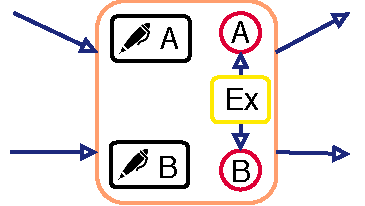
\includegraphics[width=0.8\textwidth]{images/exchange_block.pdf}
        \caption{Conceptual representation}
        \label{fig:exchange_block_conceptual}
    \end{subfigure}
    \begin{subfigure}{0.49\textwidth}
        \centering
        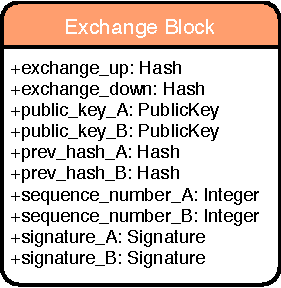
\includegraphics[width=0.6\textwidth]{images/exchange_block_data.pdf}
        \caption{Exchange block, data}
        \label{fig:exchange_block_data}
    \end{subfigure}
    \caption{A single exchange block for the TrustChain fabric. Source: \textit{Adpated from TU Delft BLockchain Lab}}
    \label{fig:exchange_block}
\end{figure}

Each agent keeps track of the actual set of blocks that were received in an exchange block such that 
the hash can be recalculated to check the validity of the exchange block. Specifically, each 
node stores an \textit{index of the blocks} contained in an exchange in a separate database. The 
index maps an exchange block to an index, consisting of the public key and sequence number for each
block received. This index can be 
used to retrieve the actual blocks from the database of blocks. This is illustrated in Figure \ref{fig:exchange_process}.

\begin{figure}
    \centering
    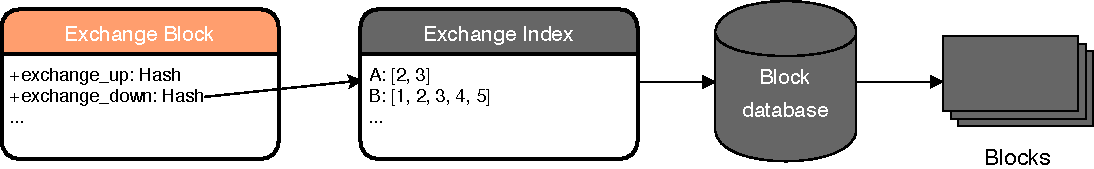
\includegraphics[width=\textwidth]{images/exchange_block_retrieval.pdf}
    \caption{Storage of exchange information: the exchange block contains a hash, which can be mapped to an index. That index can be used to retrieve the blocks from the block database.}
    \label{fig:exchange_process}
\end{figure}

\subsection{Verification protocol}
The architecture is designed in a way that another node can validate the correctness of an exchange
block. Similar to the verification of transaction blocks described in Section \ref{sec:validation} an 
exchange block sequence numbers, public keys, previous hashes and signatures need to be correct. 

Additionally, the hashes stored in the \verb|exchange_down| and \verb|exchange_up| need to be valid.
An agent $A$ is able to validate an exchange between $B$ and $C$ by requesting from $B$ the blocks 
that $B$ received and from $C$ the blocks that $C$ received. If $A$ calculates the hash of $B$'s blocks
and it add up to the hash stored in the \verb|exchange_down| and the same is true for $C$'s blocks and
the \verb|exchange_up| field, the block is valid. At this point $A$ has also established that $B$ 
and $C$ actually stored the blocks. When $A$ is only interested in confirming the honesty of one 
agent, for example $B$, $A$ can verify only the hash of the \verb|exchange_down|.

In order to validate all exchanges of one agent, the validator needs to acquire all blocks ever 
received by another agent. 

\subsection{Storage commitment}
An agent is committed to store the data that he received. As we have shown in this section any agent
$A$ can verify another agent $B$'s exchanges. The verification can only be successful if $B$ can 
summon the correct blocks. Exchanges are stored on the append-only chain where they cannot be 
removed. They can thus be verified also long after the exchange has taken place. In order to pass
verification at any time, $B$ will need to have a long-term storage for all blocks received in 
exchanges.

\subsection{Tamper-evidence and authenticity of blocks}
The tamper-evident property is inherited from the TrustChain architecture discussed in 
Section~\ref{sec:tamper-proof}. If a block is tampered with the original signatures of the block 
will be invalidated. Also any possible consecutive block's hash pointer will also be invalidated.

\section{Implementing an exchange policy}
In TrustChain the exchange behavior of agents was not visible. With the addition of exchange blocks
agents can base their decisions, for example whom to interact with, on how much data 
peers exchanged in the past. But making the gossiping behavior visible can only be the first step. 
The next step is naturally to apply the exchange records to work towards a safer distributed system.

In our model from Chapter \ref{chap:model} we defined exchange policies, which 
ensure a certain exchange of information about transaction between agents. We now consider how the
Network-State-Exchange can be implemented using the architecture defined previously. 

\subsection{Conceptual}
According to our definition an exchange policy is a set of information exchanges that are required
to be recorded, given a set of interactions. In practice this means, an agent can be required to 
first exchange information with the partner or the partner's last five partners. Specifically, the
Network-State-Exchange policy requires two agents to exchange all blocks prior to an interactions.

This strategy combines many convenient guarantees. Firstly, according to our analysis in Chapter 
\ref{chap:model} securing against a double-spend attack requires agents to obtain information. 
Secondly, given the architecture of TrustChain it is important to obtain information about the 
history of partners to assess their trustworthiness. Obtaining the complete chain of the partner 
and recording the exchange ensures that agents cannot claim to not be aware of any manipulations of 
their partners. Verifying the chain of partners becomes important because missing a manipulation
will result in becoming a fraud oneself. Finally, by exchanging all data both agents can proof to 
each other that all required data of past interaction partners was obtained and verified. Agents are
able to verify their partners complete history such that any misbehavior can be detected. 

Each agent becomes a witness of their interaction partners. Through signing the exchange of all 
information they commit to storing and disseminating that information to future interaction partners.
By signing a transaction after the exchange agents commit to having verified the information of their
partner.

\subsection{Completeness of exchange}
An obvious challenge of our architecture is how to ensure that agents actually act according to the
exchange policy. We claim that any honest agent is able to verify that their partner exchanged all 
information.

An honest agent $A$ exchanges blocks with $B$. $B$ sends his blocks to $A$ which includes his chain
and a block index for each exchange block on the chain. 
$A$ adds the received blocks to her database. If $A$ is now able to recalculate all exchange hashes
of the exchange blocks on $B$'s chain, using the block indexes and her own database, $A$ can be 
sure to have all blocks that $B$ has.

\subsection{Auditing}
We have shown in Chapter \ref{chap:model} that the Network-State-Exchange policy allows any honest
agent to re-evaluate any past verification of their partner. We will now describe this process, which
we call auditing.

An honest agent $A$ has exchanged blocks with $B$ and verified the completeness of their exchange.
$A$ therefore has all blocks that $B$ has. $A$ can then rebuild $B$ subjective network state, that
is the block database of the agent, at each exchange and interaction. Going through the chain of $B$, 
for each exchange block with some agent $C$, $A$ adds the blocks to the temporal subjective network
state of $B$ and checks whether $B$ was able to recalculate the exchange hashes of $C$'s exchange
blocks. Also $A$ checks whether all of $C$'s blocks are in that temporal subjective network state
and whether they are valid.
For every transaction block with some agent $D$, $A$ checks whether there was a valid exchange with 
$D$ prior to that transaction. 

If all verifications pass, $A$ has established that $B$ has throughout his complete history acted 
honestly. 

\subsection{Unresponsive agents}
Each honest agent will require an exchange with their partner prior to an interaction. If an agent 
asks a partner to send the blocks for an exchange it is possible that the partner does not respond.
This can either mean that the partner is not in the possession of the correct blocks to pass the  
verification and does not respond to not be exposed. On the other hand an agent can also be 
temporarily disconnected from the internet and therefore not able to respond.

The ambiguity of not responding is not problematic for our solution. Any failure to respond will
lead to no further action and therefore no transaction. If however an honest agent will at some 
point respond, the verification process is continued as normal.

\subsection{Efficient exchange}
Up to now we have considered that agents send all their blocks to each other. A simple efficiency 
improvement can be put in place such that only those blocks are sent which the partner does not have.

Given an agent's chain and the indexes that record which blocks were received in each exchange, any
other agent can create a complete index for the database of the other agent. That index is calculated
by combining the indexes of all exchange blocks and adding the transactions on the chain. The same
can be done for the agent himself. The difference between the two indexes are the blocks that one
agent has, but the other does not. During an exchange an agent can then specifically request only
those blocks.

\subsection{Exchange process}
We shall now describe the complete process of an exchange between two agents in detail. Thus, $A$ 
initiates the exchange by sending $A$'s complete chain to $B$, together with a block index for each 
exchange block.
$B$ can perform simple checks on the chain, for example whether it contains the correct number of exchange blocks
according to the exchange policy and whether all blocks are correctly signed and chained. From the 
chain and the exchange block indexes, $B$ is able to reconstruct the complete database index of $A$.

Given $A$'s database index, $B$ can calculate the difference between their databases. $B$ will 
then request from $A$ the blocks that $A$ has but $B$ does not. Once $A$ replies, $B$ has all 
information that $A$ has. $A$'s subjective network state has become transparent to $B$. 

$B$ is then able to perform the audit of $A$. If $A$'s chain completely checks out, $B$ sends his chain, exchange
indexes and blocks to $A$. Note that $B$ already knows which blocks $A$ is missing with respect to 
$B$ and can therefore directly send them. 

Now $A$ is able to perform the same checks as $B$. If $B$'s data also checks out, $A$ will create 
a new exchange block. The exchange block contains the root hash of the blocks that $A$ uploaded to $B$ 
and downloaded from $B$. As $B$ also knows which blocks he downloaded from $A$ and uploaded to $A$, $B$ should
be able to calculate the same hashes. After both parties sign the block, they add them to their 
database of blocks. Also they create an entry for the exchange block in the exchange index map, which 
maps each exchange block to the index of exchanged blocks. At this point they have concluded the 
exchange according to the Network-State-Exchange policy.

\subsection{Scalability concerns}
Each exchange between agents adds an additional block to their chain. Also, the blocks that the 
exchange contains need to be transmitted and stored. This increases the bandwidth and storage 
requirements. However, the main property of linear scalability 
still applies, at least when assuming that storage capacity is not a problem. Each exchange and 
transaction still only requires two agents to communicate, thus parallel transactions are still 
possible and the example given in Section \ref{sec:trustchain_scalability} applies in the same way.
Problems occur when we include the storage requirement. For example, the Network-State-Exchange policy
requires agents to exchange all blocks with each transaction partner. Thus each agent that periodically
interacts will approach the complete network state. Depending on the agents transaction frequency and
the network's frequency there is a considerable delay between the subjective agent's state and the
network state. Still, this will lead to storage problems if agents need to run on personal computers
or even mobile devices.

\section{Example}
In order to make the implementation more clear, an example is provided in this section. We look at two
agents, Alice and Bob. Alice wants to interact with Bob and starts the interaction. We assume that
both agents are new to the network and only have their genesis blocks on the chain. In order to
start the interaction, Alice sends her chain (only the genesis block) and an empty set of exchanges
to Bob. Obviously the genesis block is accepted and Bob shows his approval by sending his own
genesis block and an empty set of exchanges. Also Alice accepts the data. Alice creates an exchange
block which includes in the field \verb|exchange_up| the hash of Alice's genesis block and in the field 
\verb|exchange_down| the hash of Bob's genesis block. Alice signs that block and sends it to Bob. 
Bob verifies that the hashes actually are correct. If Bob agrees, he also signs the block and returns 
it to Alice. Alice also stores a block index for the created exchange block which includes as entry 
only Bob's block with sequence number 1. Similarly, Bob documents that he received Alice's first block
in the new exchange block.

At this point both agents are sure that they are honest and are able to interact in the 
application context. For example, Alice could not stream a video from Bob. After the transaction in 
the application context, Alice creates and signs a transaction block and sends it to Bob who replies 
in a similar fashion if he agrees. Figure \ref{fig:exchange_example} shows the chains of Alice and 
Bob after the complete interaction. 

\begin{figure}
    \centering
    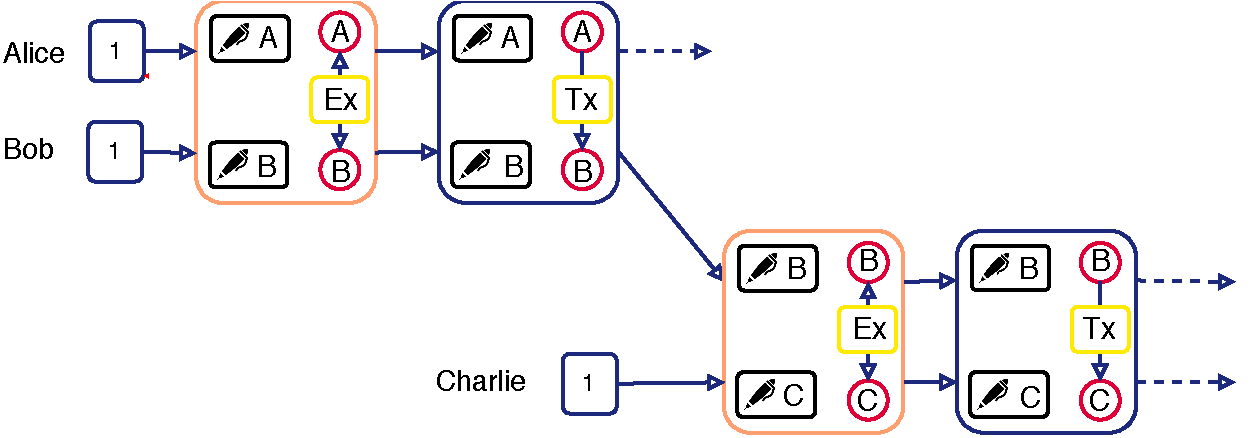
\includegraphics[width=\textwidth]{images/trustchain_example.pdf}
    \caption{Example of three agents interacting}
    \label{fig:exchange_example}
\end{figure}

This example sheds light on the block creation process but is too simple to properly explain the 
exchange and verification process. We extend the example with another agent, Charles, whom Bob would
like to interact with after the previous interactions. Again, Charles is assumed to be new to the 
network so the genesis block is the only block on his chain. Bob starts the interactions by sending
his chain and the index that documents the acquisition of Alice's first block. 

Charles sees that Bob has an exchange block with Alice before have a transaction with her, which is 
correct according to the exchange policy. Next Charles checks the signatures and hashes of Bob's chain. 
After those checks pass, Charles tries to calculate the hashes for Bob's exchange block but realizes
that he does not have Alice's first block. Therefore he requests it from Bob. After receiving it the
check should pass. 

Once Charlie accepts all the checks, he sends his own chain and exchanges which are checked by Bob
and the interaction continues as previously described. Table \ref{tab:blocks_example} shows the
blocks that each agent has after the first and second round. After the second round, Charles has 
all the blocks from Bob that he had after the first round.

\begin{table}[h!]
    \centering
    \caption{The block databases of each agent for the example}
    \label{tab:blocks_example}
    \begin{tabular}{p{4cm}|p{3cm}|p{4cm}|p{3cm}}
        \toprule
        Database & Alice & Bob & Charles \\
        \midrule
        Before first round & A: $[1]$ & B: $[1]$ & C: $[1]$ \\ \hline 
        After first round & A: $[1, 2, 3]$ \newline B: $[1, 2, 3]$ & A: $[1, 2, 3]$ \newline B: $[1, 2, 3]$ & C: $[1]$ \\ \hline
        After second round &  A: $[1, 2, 3]$ \newline B: $[1, 2, 3]$ & A: $[1, 2, 3]$ \newline B: $[1, 2, 3, 4, 5]$ \newline C: $[1, 2, 3]$ & A: $[1, 2, 3]$ \newline B: $[1, 2, 3, 4, 5]$ \newline C: $[1, 2, 3]$ \\
        \bottomrule
    \end{tabular}
\end{table}


% \subsection{Obtaining a subject network state}
% One property of the extended architecture that we proposed in this section is that an agent's complete
% database is transparent to other nodes. It enables nodes to explore another node's view of the network. 
% In our model we called this the subjective network state. 

% Specifically, a node $A$ obtains a complete
% chain from an agent $B$ which includes transaction and exchange blocks. Furthermore, for each exchange 
% $B$ provides $A$ with the index of blocks contained in that exchange. If $A$ is able to recalculate 
% all the exchange hashes stored in the exchange blocks of $B$, $A$ has at least all information that 
% $B$ has and is able to obtain an exact similar subjective network state as $B$. If not, $A$ can see 
% from the exchange indexes which blocks $B$ has that $A$ does not. $A$ can request those from $B$, and
% if $B$ is honest $B$ will respond. Finally, 


% Exchange policies allow the system designer to ship software with a less or more stringent
% exchange policy. This will reduce or increase security but also impact the requirements on storage and bandwidth.
% If a stringent policy is applied, it should be possible to delete data. This could also be recorded on chain. As only the 
% root hash of the exchanges are stored on an agents chain, a delete block should be possible by 
% recording in a similar fashion without the need to remove blocks from the chain. Therefore chain 
% consistency is kept intact. How this should be implemented in detail and a security analysis will 
% be left for future research.

\section{Other exchange policies}
\label{sec:system_trust}
The architecture that we have presented in the previous section is very flexible. Any size of information 
exchange between two parties can be recorded. It therefore allows for the implementation of any 
exchange policy. We described in the previous section how the Network-State-Exchange policy can be implemented
and that it can give strong guarantees for security but also induces the highest cost on storage and bandwidth 
capacity. Depending on the application this might be necessary however TrustChain was designed to 
be as scalable as possible without global consensus. Therefore also less demanding exchange policies
can be implemented.

Instead of enforcing a certain policy, the exchange records can also be used to create a system level 
notion of trust. We have extensively introduced the concept of trust in Chapter~\ref{chap:introduction} and discussed
how it plays a role in different contextual settings. Afterwards we have mostly considered trust in 
an application context like Tribler. TrustChain records transactions between users in the application
context which act as evidence of a user history. That history is used to calculate a reputation and
ultimately a trust value for each known user. Yet, the architecture of TrustChain and even more so 
the architecture of the extended TrustChain make room for another concept of trust on a system level.

Each agent in the system engages in recording, exchanging and verifying behavior. Agents do this 
with a certain reliability. Until now we assumed that agents are either perfectly honest, malicious
or free-riders, so there was no forgiveness and no shades of honesty. That is fine when considering
automated agents in a theoretical setting, however in practice this may not be realistic or 
desired. Instead we could assign a reputation to agents based on their exchange and verification 
behavior which is increased with ``positive'' action like exchanges and decreased with any 
``negative'' evidence, like multiple interactions without exchanges. Also, if we consider the way 
we defend against verification free-rider as described in Section \ref{sec:verification_free-riding}, 
agent completely redo all verification of an agent in order to verify that the agent behaved correctly.
Trust at system level could create a relationship between agents such that they can rely on each 
others' verification of peers. 

% \section{Attacks}
% We now consider possible ways to attack the 

% \subsection{Block tampering}
% Similar to the block tampering that we described in Section \ref{sec:tampering}, an agent could 
% directly change the hash of received blocks after an exchange. Again, the signature of the partner 
% stored in the block will be invalidated. 

% \subsection{Not actually storing information}
% The information that is received is only recorded in form of the root hash of contained blocks. The 
% actual blocks are in the database of the agent itself which is obviously opaque to other agents. 
% Therefore an agent $A$ could possible only record correctly the exchange but not actually store the 
% received information. 

% However, other agents are expecting $A$ to be in the possession of the block. Thus, depending 
% on the exchange policy, an agent might at some point request a block in which case $A$ is not able 
% to respond. This will expose the agent of free-riding on the storage.

% \paragraph{Collusion}
% As we have previously discussed in Section \ref{sec:collusion}, attacking agents can work together in 
% a collusion attack. We claim that a subset of those collusion attacks is more difficult if agents are
% able to obtain subjective network state transparency. Consider two agents $A$ and $B$ are colluding 
% in a block tampering. $B$ has changed a block in order to obtain more reputation and $A$ is transacting 
% with $B$ to receive some of the maliciously gained reputation. But in order to transact and be considered
% an honest agent, $B$ needs to obtain $A$'s chain. In that case 

% * Verification and exchanges make an agent trustworthy on a system level, as in, we trust them to 
% stick to the rules of recording, exchanging and verifying
% * Use this to not verify each and every agent, but assume agent which were verified by trustworthy
% agents to be trustworthy enough for interaction
% * At every point we still have the chance to do the complete verification of a history. But maybe 
% its not required every turn

% \chapter{Reputation consensus through anti-entropy}
\label{chap:mechanism}
% A specific implementation of the extension of TrustChain

% A policy that makes dissemination and verificaiton strategy-proof
In the first chapters of this thesis we introduced the incentive problem of information dissemination 
in distributed reputation systems. In the previous chapter we introduced an extension of the TrustChain
architecture that allows for agents in the network to obtain and verify each other's internal 
information state. But in order to achieve the goal of strategy-proof dissemination of information
a tangible mechanism is required that applies the advanced tools that the new architecture provides.
In this chapter we analyze one such mechanism which is based on the anti-entropy concept. We first
describe the mechanism conceptually, then discuss the implementation details and finally elaborate
on some intrinsic properties the mechanism could introduce in actual applications. In the next
chapter an implementation will be analyzed experimentally with small agent sets in order to prove
that properties from the theoretical analysis can be observed in practice.

\section{Conceptual description}
% The exact protocol: before each transaction we exchange all data and verify each other's chain

% What this allows us to do is: we can agree on a ranking that includes all of both agents data. 

% We give the receiver a chance to proof that he is worth

% We make sure that an agent has to obtain all data before making a transaction. 
Section~\ref{sec:strategy_proof_sharing} explained that the architecture itself does not solve the 
incentive problem. It rather provides the evidence on which an incentive mechanism can be built. 
Many different mechanism are possible, depending on the specific needs of the application context. 
This offers a lot of flexibility for system designers which is different from existing architectures
which a very static in their protocol and have pre-defined security and scalability properties.

\subsection{Design choice: security vs scalability}
Security, decentralization and scalability are three properties that are traded against each other 
in the design of a decentralized system. It can be argued that TrustChain was designed with scalability
as the highest priority while Bitcoin was designed with security as highest priority property. We
argue that the extension that allows for internal agent state transparency allows for flexibility in
the design choice of security and scalability. In this section we propose a mechanism that trades 
some of the scalaiblity of TrustChain for stronger security in order to show that a secure mechanism
is possible on top of the TrustChain architecture. 

\subsection{Concept: anti-entropy}
The mechanism is based on the concept of anti-entropy, which was described in \cite{demers1987epidemic}
for the purpose of maintaining mutual consistency between multiple replicas of a database. Updates
to the database can arrive at any single site and need to be forwarded to all other replicas. Demers
et. al. study three different mechanisms to disseminate the updates to other sites: direct mail, 
anti-entropy and rumor mongering.

In the direct mail mechanism, a database forwards the update to all other database immediately, which
seems like the most straight forward approach but is restricted by the fact that each database does
not know about all other databases. 

Anti-entropy is a process in which each database periodically chooses a partner database and both 
exchange all database contents in order to resolve any differences between the two. The process was
found to be reliable but slower than direct mail. 

The final mechanism is called Rumor Mongering. Sites consider updates ``hot rumors'' after receiving
them for the first time. While the site considers the rumor ``hot'', it choses periodically another
site and informs it about the rumor. When the site has encountered a certain amount of sites which
were already aware of the ``hot rumor'', that update is retained but site stops with actively
propagating the update. 

For the purpose of this work, we will focus on the concept of anti-entropy. Direct mail is not a
viable option because for large social networks the embedded social networks are a very small 
subset and the rest of the agents in the network would not be informed of updates. Rumor mongering 
effects are best observed in larger networks however this work is concerned with conceptual analysis
and the experimental analysis in the next section concerns small networks. Also there are more 
algorithms than these three but anti-entropy fits the architecture of TrustChain very well and is 
a good starting point for analyasis of dissemination mechanisms. The analysis of other mechanisms
will be subject of future work.

\subsection{Replicated databases vs TrustChain}
The context of the work of Demers et. al. is similar to the context that this work is concerned with
in many regards. Replicated databases are a distributed system as all instances of the database are
independent, equal entities, just like the agents in the TrustChain network. Each agent has an 
internal state which is equal to the set of transactions that agent is aware of which is equal to
the state of the database which is equal to the entries that database is aware of. Our goal is to 
propagate information on new transactions just like the goal of Demers et. al. was to propagate 
updates to the databases. 

In the context of reputation systems anti-entropy allows for two agents to align on their knowledge
of the social network, that is to obtain the same embedded social network and agree on the reputation
of all agents in that network.
Two agents, $a_i$ and $a_j$ have two different internal states, represented by the sets of encounters
$E_i$ and $E_j$. There can be some overlap between the two sets, but that is not guaranteed. Agent 
$a_i$ chooses to synchronize states with agent $a_j$. Both agents send their own set of known 
encounters and merge them. This results in a new set $E_{i,j} = E_i \bigcup E_j$. In the context 
of TrustChain this translates to the exchange of transaction blocks, such that after the exchange 
both agents have the exact same set of transaction blocks. As the reputation of peers is calculated
from the set of transactions both agents agree on a single reputation vector. If the two agents also
use the same function for trust calculation both can even agree on a single trust vecotr. The two 
agents have reached consensus on trust and reputation. 

The exchange of information will be recorded in the form of exchange blocks on the chain of both 
participating agents as explained in the previous chapter, section~\ref{sec:implementation_state_transparency}.

The consensus is only reached at one point in time and is not maintained. Once any of the two agents
conducts another anti-entropy exchange or a transaction, the other agent is not required to be 
informed or to observe the interaction. That is after the exchange both internal states can diverge
until the same two agents happen to perform another state synchronization. 

In the work of Demers et. al. database instances chose partners for anti-entropy exchanges at random
which is a valid strategy as each peers updates seem equally important. In contrast, reputation 
systems should value the information about possible future interaction partners as more important.
Therefore, our proposed mechanism requires agents to at least perform an anti-entropy exchange with
those agents that they will have an interaction next. That way, both parties of a transaction are 
required to obtain and verify each others information in order to make sure that the transaction 
will be done on top of a valid state. If any party does not agree with the state of the opposite 
party, the transaction will not take place. If any party performs a transaction eventhough the 
information clearly shows misconduct on the part of the partner, they will also be held responsible 
for not performing their validation responsibility. Without the requirement of validating transaction
partners, agents can purposefully exchange data with honest agents but perform interactions with 
dishonest agents and later claim to have had no knowledge of the dishonesty of the partners. 

\section{Implementation of anti-entropy exchanges}
In the previous section we described the anti-entropy method for information exchanges between 
agents. This section elaborates on the implementation details of the mechanism in the TrustChain 
architecture. We start with an application agnostic example of the exchange of information and the 
transaction process.. In the next section we expand on the considerations for application specific 
implementations.

We consider an agent $a_i$, who is about to conduct another interaction. What the interaction is 
about and how the partner is chosen are specific to the application context. For this example we 
assume that $a_i$ can randomly choose an agent from the network. Once $a_i$ has chosen a partner $a_j$,
$a_i$ starts the communication and is therefore the \textit{initiator} while $a_j$ is the \textit{responder}. 

The initiator starts the interaction by sending the chain and exchange history to the responder. The
chain{\color{red} Is this explained somewhere} includes the blocks that describe the transaction and 
exchange history {\color{red} Is this explained somewhere} of the initiator while the exchange 
history includes the index of blocks exchanged for each exchange block. On reception, the responder 
can verify the chain using the algorithm \ref{alg:verify_chain}. The algorithm first checks,
wether the chain is a complete sequence without missing blocks in between. If the check is positive,
the number of exchange and transaction blocks is compared, as well as the public keys of partners
such that each transaction can be paired with a succesful exchange previous to the transaction.

\begin{algorithm}
\caption{Chain }\label{alg:verify_chain}
\begin{algorithmic}[1]
\Procedure{verifyChain}{}
\EndProcedure
\end{algorithmic}
\end{algorithm}

Once that check also succeeds, the responder is able to build a block index that indexes the internal
state of an agent. The block index is a summary of the contents of the internal state and shows
which transactions of which agents are knwon to the agent. This is an optimization that allows agent
to request only specific blocks instead of the complete database of another agent. This is a lot 
faster if agents that already share a lot of data. Agent $a_j$ compares the calculated block index
with his own index and request the difference in blocks, so those that $a_i$ has but $a_j$ does not 
have from $a_i$.

The initiator receives the request and replies with the blocks that $a_j$ requires to perform the 
complete internal state validation. Should the responder, for whatever reason, wrongly require more
blocks, so also blocks that are not in $a_i$'s posession, the interaction will be canceled. 

The responder receives the missing blocks. At this point $a_j$ should be in the posession of all
of $a_i$'s blocks plus some blocks that $a_j$ has over $a_i$. Agent $a_j$ is then able to perform
the complete internal state verification according to algorithm~\ref{alg:verify_state}. A state is
valid if:

\begin{algorithm}
    \caption{Chain }\label{alg:verify_state}
    \begin{algorithmic}[1]
    \Procedure{verifyChain}{}
    \EndProcedure
    \end{algorithmic}
\end{algorithm}

\begin{itemize}
    \item the chain is valid as per algorithm~\ref{alg:verify_chain}
    \item the hashes of the blocks according the the exchange indexes match the hashes recorded on
    the chain's exchange blocks
    \item Any recorded misbehavior of other agents is reflected by those agents' public keys in the 
    ignore and block list
\end{itemize}

If the internal state of $a_i$ is determined to be valid by $a_j$, the responder shows approval by 
sending the own chain, exchange history and blocks (which can be calculted by taking the opposite
difference from before) to agent $a_i$. 

Once the initiator receives that data from the responder, the second validtion of chain and state, 
this time agent $a_j$ as subject, can be conducted. If also this checks out, the valdiation phase is 
completed and the initiator can publish an exchange block proposal, which includes the hashes of the
exchanged blocks. The responder receives that proposal and the hashes contained in the proposal block
match the hashes that $a_j$ calculates for the excahnged data, the block is signed and returned.

This concludes the anti-entropy exchange, after this the two agents perform a normal interaction.

\section{Consideration of application specific features}
choosing partners -- we now chose partners randomly but probably for many applications there are 
better strategies
application specific rules -- we could perform addiitonal verification for application context, for
example no downloading after a certain negative balance boundary

\section{Advanced implicaitons of anti-entropy}
locality -- when you need to exchange all information and storage has avlue, it is cheapter to 
interact with agents that have a largely similar information set
sybil attack -- when we can apply application specific rules and we require agents to perform checks
of all agents they interact with, we can introduce a rule that says agents cannot upload to agents
that are completely new to the network (they first have to prove themselves). This way an agent 
cannot create fake agents that all download from one agent and thus increase that agents balance 
without actual downloading happening


\chapter{Experiments and results}
Theory shows that internal agent state transparency and the anti-entropy mechanism reward honesty
and punish any strategic manipulation. We implemented this mechanism and establish in this chapter
how it handles strategic manipulation. More specifically we emulate honest agents and multiple 
types of strategic manipulators in small scale experiments. We can observe the behavior of the 
honest agents and find that strategic manipulators are detected and isolated. We show that honest agents who
execute our mechanism are able to effectively detect malicious agents that do not share or do not verify their partners 
and ignore them for future interactions.

The rest of the chapter is structured as follows: we first give an overview of the software 
architecture. Then we explain the setup of the experiments and the types of strategic manipulation
that will be emulated. Finally we present the results of the experiments.

% In the previous chapters we have explored the problem of dissemination of information in distributed
% trust systems. We offered a solution in the form of our multichain based TrustChain architecture, extended 
% it with internal agent state transparency and designed a mechanism that prevents any free-riding on
% dissemination and validation of information on transactions. In this chapter we aim to prove the 
% properties of the mechanism and architecture by experimental analysis. We built a proof-of-concept
% software that fully implements the architecture and mechanism described in this work. It allows us 
% to run an emulation of an agent network and study the behavior of agents in the presence of strategic
% manipulators.

\section{Experiment design}
The goal of the experiments is to prove the true effectiveness of the mechanism at detecting 
manipulation attempts and isolating malicious agents. Three different types of dishonest behavior 
will be analyzed in the experiments.

\begin{itemize}
    \item \textbf{Dissemination free-rider}: An agent that performs transactions normally but does
    not respond to exchange requests or start own exchanges.
    \item \textbf{Validation free-rider}: An agent that performs exchanges and transactions normally
    but does not perform any validation
    \item \textbf{Forking}: An agent creates two conflicting transactions and forwards them to two 
    different partners without telling them about the other transaction.  
\end{itemize}

% The goal of the experimental analysis is to show that free-riding on dissemination and validation of
% transaction information is no longer possible with the extension of TrustChain proposed in 
% chapter~\ref{chap:state_transparency} and the mechanism in chapter~\ref{chap:mechanism}. This would
% be a major step towards a secure and valid distributed trust system. 

In the experiments we emulate small agent networks up to 6 agents. We assume that agents are trying to perform 
interactions with each other. The experiments are not concerned with the actual trust agents have 
in each other so we keep transaction blocks empty. Agents are acting completely autonomously 
but knows about all the other agents in the network. At a frequency of 20 per second agents go through
rounds, in each round an agent has a 1\% chance of starting an interaction. This adds up to approximately
1 transaction every 5 seconds. In addition agents respond to interaction requests from their peers 
asynchronously. At the start of the interaction a peer is selected with uniform probability. If an
interaction with the selected partner is already ongoing, the new interaction request is cancelled
without selecting a new partner. The same happens when the selected partner is a known malicious 
agent. Once the interaction is started honest agents perform according the mechanism as described in
chapter \ref{chap:mechanism}. The other types of agents each have some deviation from the expected
behavior in order to obtain an unfair advantage.

\begin{itemize}
    \item \textbf{Dissemination free-rider}: An agent that performs transactions normally but does
    not respond to exchange requests or start own exchanges.
    \item \textbf{Validation free-rider}: An agent that performs exchanges and transactions normally
    but does not perform any validation
\end{itemize}

With these types of agent we run experiments with different sets of agents. In experiments with only
a single dishonest agent, the experiment is successful if the honest agents stay among themselves
and ignore the dishonest agent. That is, the dishonest agent should have 0 transactions at the end
of the experiment. In the case with multiple dishonest agents we have to make a distinction between
multiple single acting dishonest agents and collaborating groups of dishonest agents. 

\section{Implementation details}

\begin{itemize}
    \item Python implementation 
    \item zermq sockets
\end{itemize}


\section{Experiment results}
\subsection{Dissemination free-riders}
\begin{figure}
    \begin{subfigure}{\textwidth}
      \centering
      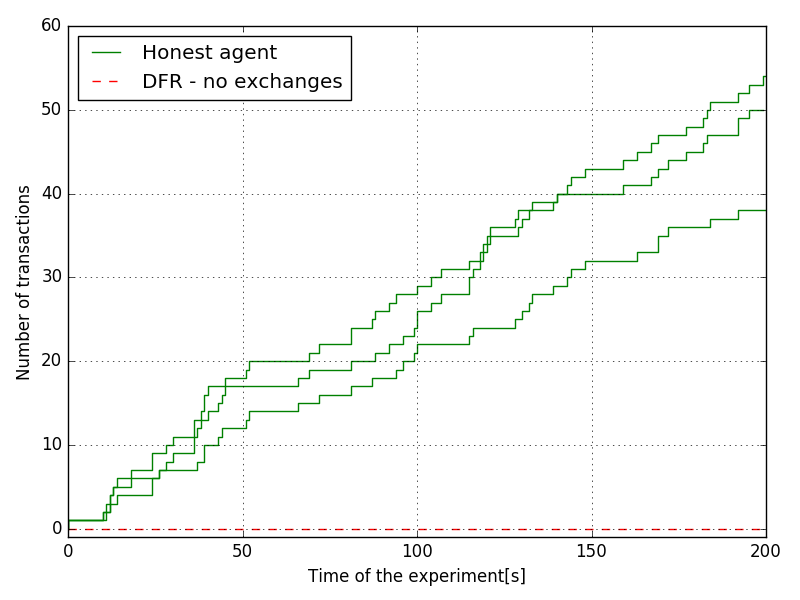
\includegraphics[width=.6\linewidth]{images/DFR_no_exchanges}
      \caption{Transactions over time of honest agents with dissemination free-rider that does not 
      perform any exchanges}
      \label{fig:DFR_no_exchanges}
    \end{subfigure}\\
    \begin{subfigure}{\textwidth}
      \centering
      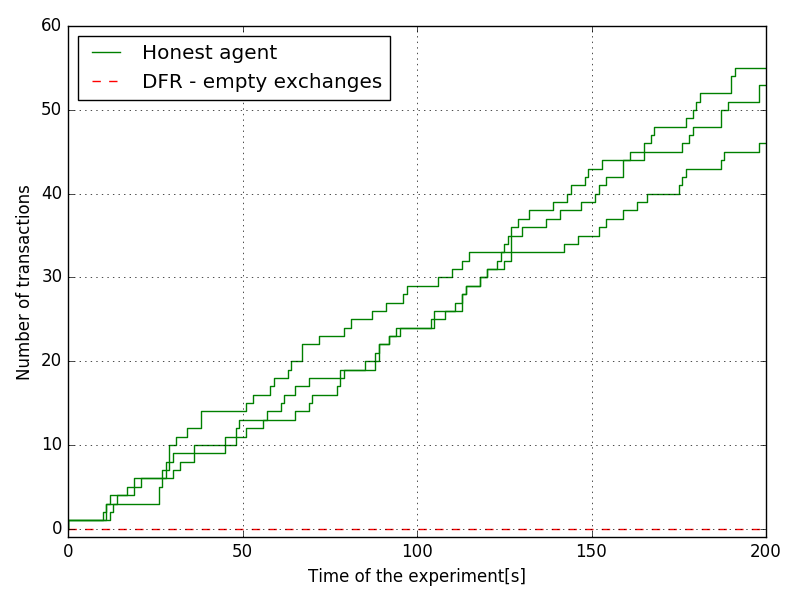
\includegraphics[width=.6\linewidth]{images/DFR_empty_exchanges}
      \caption{Transactions over time of honest agents with dissemination free-rider that creates 
      empty exchanges}
      \label{fig:DFR_empty_exchanges}
    \end{subfigure}\\
    \begin{subfigure}{\textwidth}
        \centering
        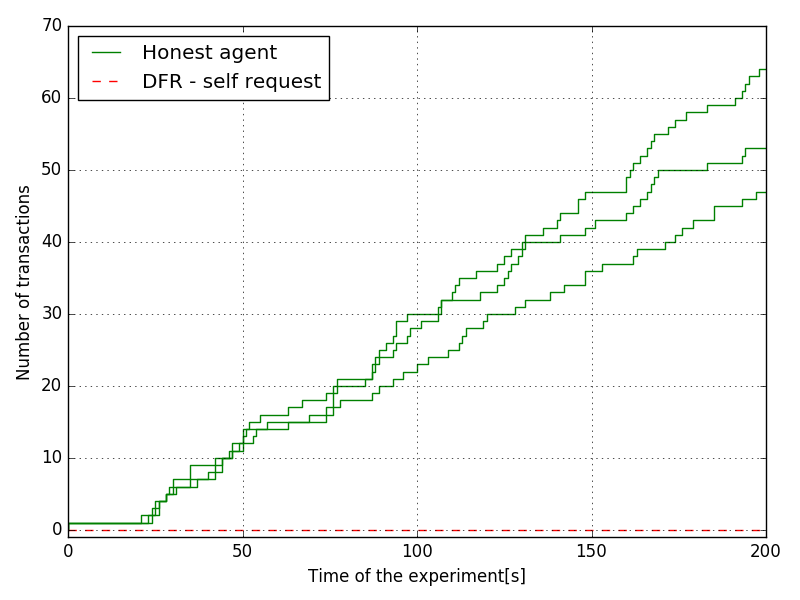
\includegraphics[width=.6\linewidth]{images/DFR_self_request}
        \caption{Transactions over time of honest agents with dissemination free-rider that only 
        exchanges own data}
        \label{fig:DFR_self_request}
      \end{subfigure}
\end{figure}

\subsection{Collaborating dissemination free-riders}

\begin{figure}[h!]
    \centering
    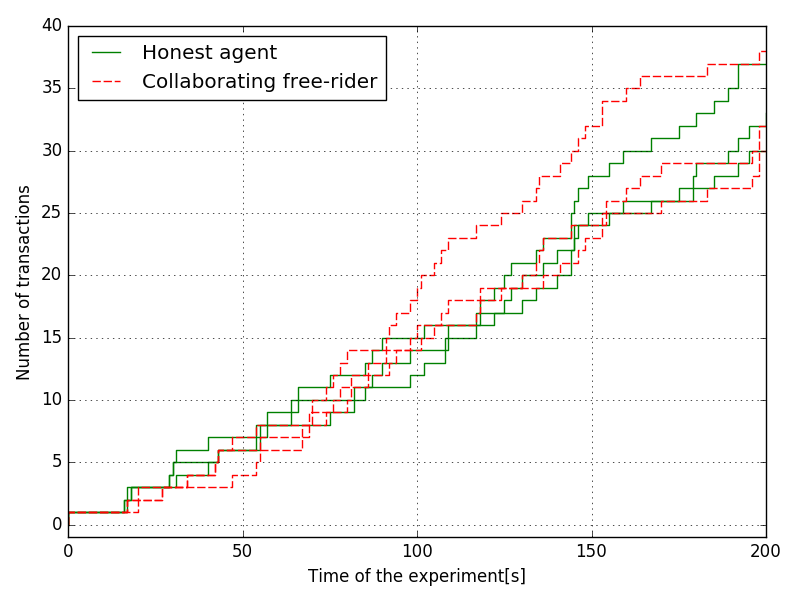
\includegraphics[width=0.7\textwidth]{images/50percent}
    \caption{Transaction history of three honest agents and three dissemination free-riders
    that are cooperating}
    \label{fig:50percent}
\end{figure}

\begin{figure}[h!]
    \centering
    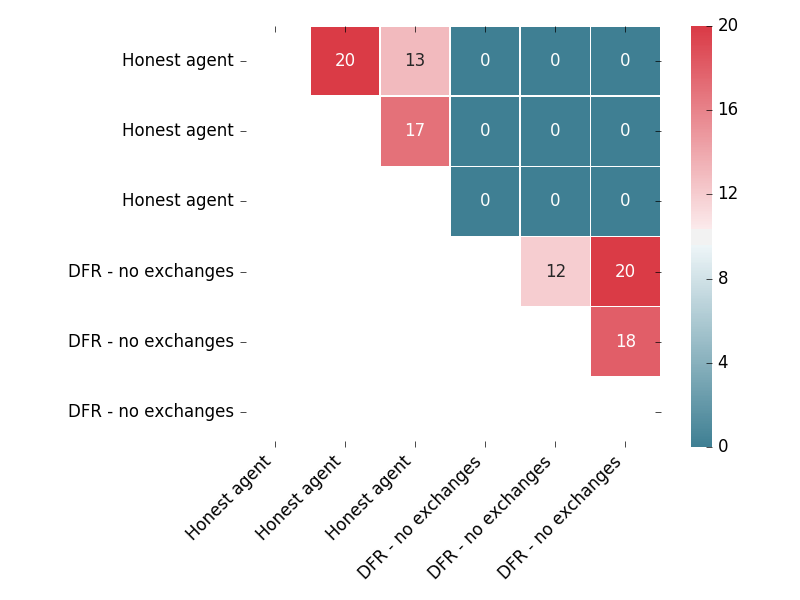
\includegraphics[width=0.7\textwidth]{images/50percent_interaction_matrix}
    \caption{Interaction matrix of three honest agents and three dissemination free-riders who are cooperating}
    \label{fig:50percent}
\end{figure}

\subsection{Malicious behavior}

\begin{figure}
    \begin{subfigure}{\textwidth}
      \centering
      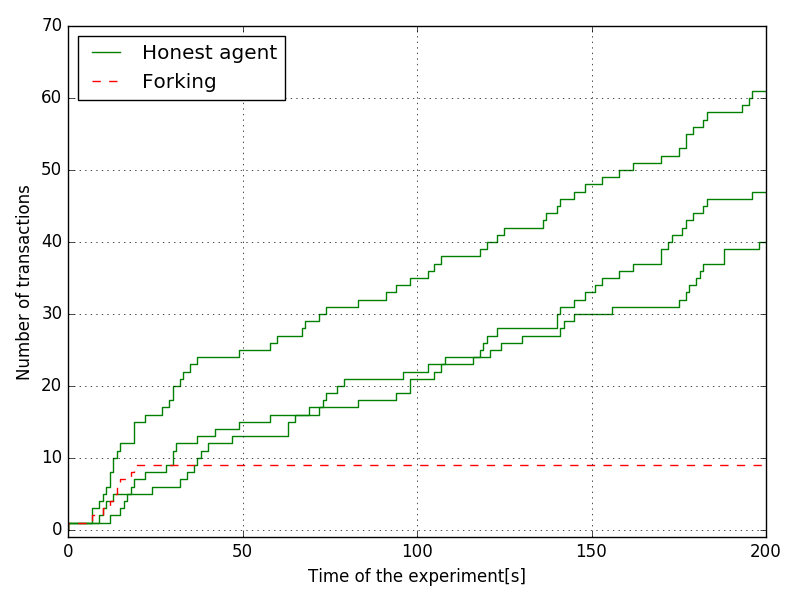
\includegraphics[width=.6\linewidth]{images/forking}
      \caption{Transaction history of three honest agents interacting with one strategic manipulator who performs a fork}
      \label{fig:forking}
    \end{subfigure}\\
    \begin{subfigure}{\textwidth}
      \centering
      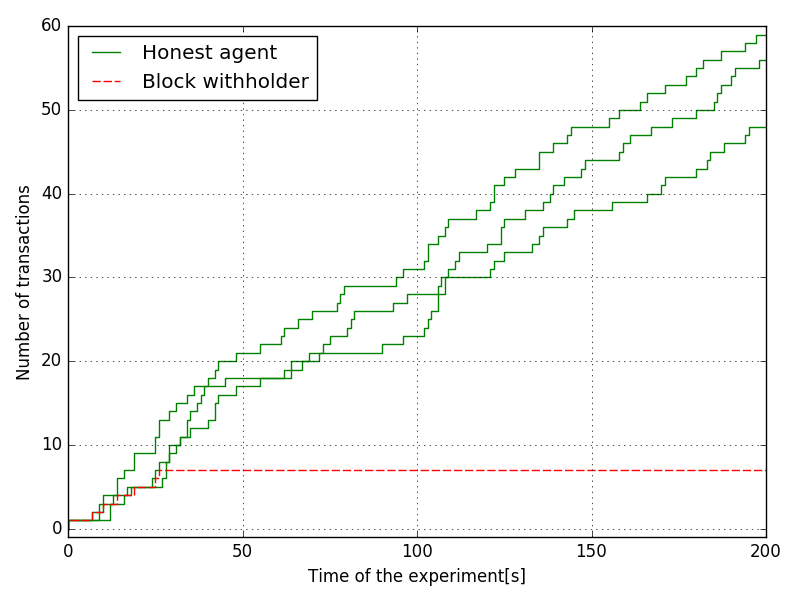
\includegraphics[width=.6\linewidth]{images/transaction_hiding}
      \caption{Transactions over time of three honest agents with one strategic manipulator who tries to hide a transaction}
      \label{fig:DFR_empty_exchanges}
    \end{subfigure}\\
\end{figure}

\subsection{Verification free-rider}

\begin{figure}
    \begin{subfigure}{\textwidth}
      \centering
      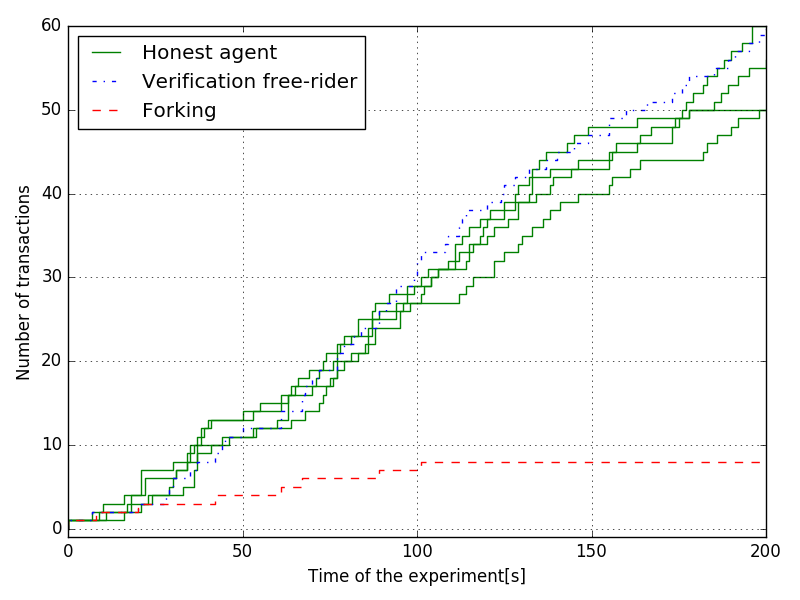
\includegraphics[width=.6\linewidth]{images/verification_doublespend_honest}
      \caption{Transaction history of three honest agents interacting with one strategic manipulator who performs a fork and a verification free-rider}
      \label{fig:verification_doublespend_honest}
    \end{subfigure}\\
    \begin{subfigure}{\textwidth}
      \centering
      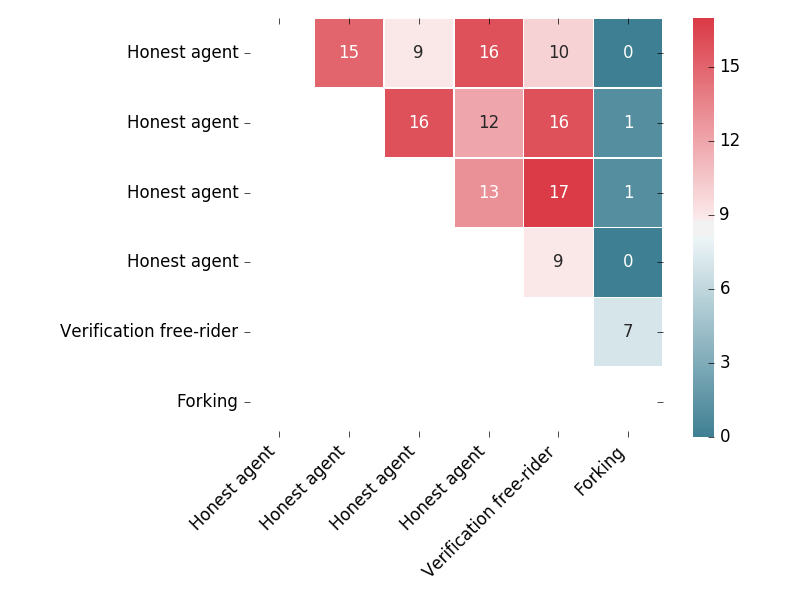
\includegraphics[width=.6\linewidth]{images/verification_doublespend_honest_matrix}
      \caption{Interaction matrix of three honest agents with one strategic manipulator who performs a fork and a verification free-rider}
      \label{fig:verification_doublespend_honest_matrix}
    \end{subfigure}\\
\end{figure}

\begin{figure}
    \begin{subfigure}{\textwidth}
      \centering
      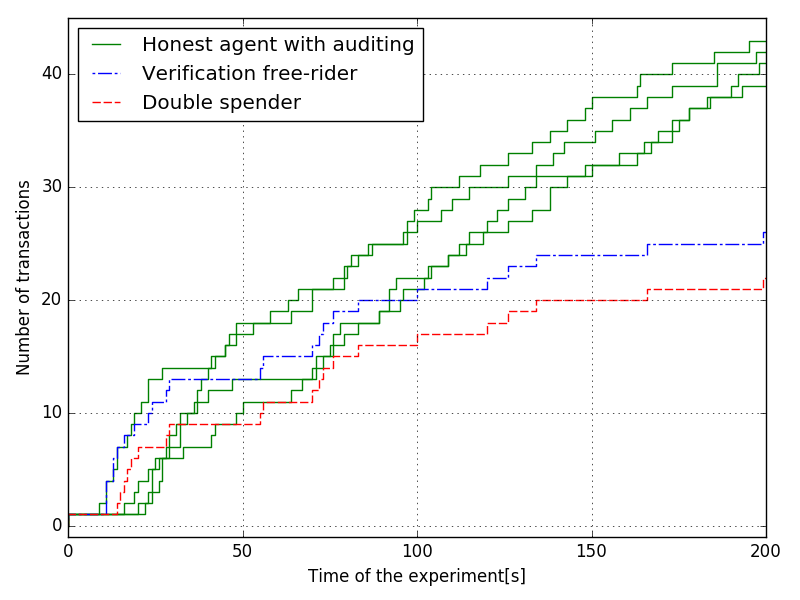
\includegraphics[width=.6\linewidth]{images/verification_doublespending}
      \caption{Transaction history of three honest agents with replay verification interacting with one strategic manipulator who performs a fork and a verification free-rider}
      \label{fig:verification_doublespending}
    \end{subfigure}\\
    \begin{subfigure}{\textwidth}
      \centering
      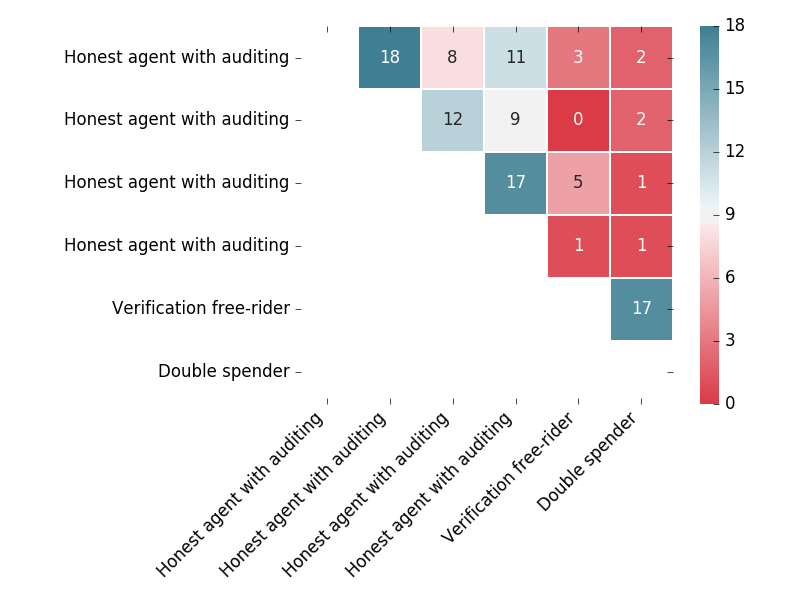
\includegraphics[width=.6\linewidth]{images/verification_doublespending_matrix}
      \caption{Interaction matrix of three honest agents with replay verification with one strategic manipulator who performs a fork and a verification free-rider}
      \label{fig:verification_doublespending_matrix}
    \end{subfigure}\\
\end{figure}

\section{}

\subsection{Sybil attack}

\chapter{Discussion}
In this work we presented a strategy-proof mechanism for information dissemination. Applied to our 
distributed blockchain based trust system we are able to effectively defend against dissemination 
and verification free-riders. It creates an incentive for each agent on the network to help defend 
the network against any lazy or malicious behavior. It thereby is a major step towards a secure, 
distributed and scalable trust system.

* we defined a new blockchain system based on TrustChain which provides internal agent state 
transparency/gossip transparency
* we formally proof that the architecture provides a complete view of the internal state of the 
agent
* we defined a specific mechanism that makes use of the archiecture
* we experimentally proof that honest agents are able to eventually identify free-riders and malicious
agents

\section{Future research}

\subsection{Further developing this mechanism}
* incremental 
* research scalability properties for this mechanism
* locality by interacting with those that have similar information
* sybil attack resistance by checking that new agents paid their dues

\subsection{Next steps for the trust system}
* locality with ping
* 

%% Use letters for the chapter numbers of the appendices.
\appendix

%\input{appendix-a}

\bibliography{report}

\end{document}

